\documentclass[letterpaper,12pt,oneside]{article}\usepackage[]{graphicx}\usepackage[]{color}
%% maxwidth is the original width if it is less than linewidth
%% otherwise use linewidth (to make sure the graphics do not exceed the margin)
\makeatletter
\def\maxwidth{ %
  \ifdim\Gin@nat@width>\linewidth
    \linewidth
  \else
    \Gin@nat@width
  \fi
}
\makeatother

\definecolor{fgcolor}{rgb}{0.345, 0.345, 0.345}
\newcommand{\hlnum}[1]{\textcolor[rgb]{0.686,0.059,0.569}{#1}}%
\newcommand{\hlstr}[1]{\textcolor[rgb]{0.192,0.494,0.8}{#1}}%
\newcommand{\hlcom}[1]{\textcolor[rgb]{0.678,0.584,0.686}{\textit{#1}}}%
\newcommand{\hlopt}[1]{\textcolor[rgb]{0,0,0}{#1}}%
\newcommand{\hlstd}[1]{\textcolor[rgb]{0.345,0.345,0.345}{#1}}%
\newcommand{\hlkwa}[1]{\textcolor[rgb]{0.161,0.373,0.58}{\textbf{#1}}}%
\newcommand{\hlkwb}[1]{\textcolor[rgb]{0.69,0.353,0.396}{#1}}%
\newcommand{\hlkwc}[1]{\textcolor[rgb]{0.333,0.667,0.333}{#1}}%
\newcommand{\hlkwd}[1]{\textcolor[rgb]{0.737,0.353,0.396}{\textbf{#1}}}%
\let\hlipl\hlkwb

\usepackage{framed}
\makeatletter
\newenvironment{kframe}{%
 \def\at@end@of@kframe{}%
 \ifinner\ifhmode%
  \def\at@end@of@kframe{\end{minipage}}%
  \begin{minipage}{\columnwidth}%
 \fi\fi%
 \def\FrameCommand##1{\hskip\@totalleftmargin \hskip-\fboxsep
 \colorbox{shadecolor}{##1}\hskip-\fboxsep
     % There is no \\@totalrightmargin, so:
     \hskip-\linewidth \hskip-\@totalleftmargin \hskip\columnwidth}%
 \MakeFramed {\advance\hsize-\width
   \@totalleftmargin\z@ \linewidth\hsize
   \@setminipage}}%
 {\par\unskip\endMakeFramed%
 \at@end@of@kframe}
\makeatother

\definecolor{shadecolor}{rgb}{.97, .97, .97}
\definecolor{messagecolor}{rgb}{0, 0, 0}
\definecolor{warningcolor}{rgb}{1, 0, 1}
\definecolor{errorcolor}{rgb}{1, 0, 0}
\newenvironment{knitrout}{}{} % an empty environment to be redefined in TeX

\usepackage{alltt}
\usepackage[paperwidth=8.5in,paperheight=11in,top=1in,bottom=1in,left=1in,right=1in]{geometry}
\usepackage{setspace}
\usepackage[colorlinks=true,allcolors=Blue]{hyperref}
\usepackage[usenames,dvipsnames]{xcolor}
\usepackage{indentfirst}
\usepackage{titlesec}
\usepackage{multirow}
\usepackage{booktabs}
\usepackage{graphicx}
\usepackage{verbatim}
\usepackage{rotating}
\usepackage{tabularx}
\usepackage{outlines}
\usepackage{lineno}
\usepackage{array}
\usepackage{times}
\usepackage{cleveref}
\usepackage{acronym}
\usepackage[position=t]{subfig}
\usepackage{paralist}
\usepackage[noae]{Sweave}
\usepackage{natbib}
\usepackage{array}
\usepackage{pdflscape}
\usepackage{bm}
\usepackage[inline]{showlabels}
\bibpunct{(}{)}{,}{a}{}{,}

% page margins and section title formatting
\linespread{2}
\setlength{\footskip}{0.5in}
\titleformat*{\section}{\Large\bf\em}
\titleformat*{\subsection}{\singlespace\large\bf}
\titleformat*{\subsubsection}{\singlespace\normalsize\bf\em}
\titlespacing{\section}{0in}{0in}{0in}
\titlespacing{\subsection}{0in}{0in}{0in}
\titlespacing{\subsubsection}{0in}{0in}{0in}

% cleveref options
\crefname{table}{Table}{Tables}
\crefname{figure}{Fig.}{Figs.}
\renewcommand{\figurename}{Fig.}

%acronyms
\acrodef{chla}[chl-\textit{a}]{chlorophyll \textit{a}}
\acrodef{din}[DIN]{dissolved inorganic nitrogen}
\acrodef{emp}[EMP]{Environmental Monitoring Program}
\acrodef{iep}[IEP]{Interagency Ecological Program}
\acrodef{jas}[JAS]{July-August-September}
\acrodef{sfe}[SFE]{San Francisco Estuary}
\acrodef{wrtds}[WRTDS]{Weighted Regressions on Time, Discharge, and Season}
\acrodef{wwtp}[WWTP]{wastewater treatment plant}
\acrodefplural{wwtp}[WWTPs]{wastewater treatment plants}

% for unit macros
\newcommand{\mgl}{mg L$^{-1}$}
\newcommand{\mugl}{$\mu$g L$^{-1}$}

%knitr options


% get the version based on commit date


% get online bib file


\IfFileExists{upquote.sty}{\usepackage{upquote}}{}
\begin{document}

\raggedbottom
\linenumbers
\raggedright
\urlstyle{same}
\setlength{\parindent}{0.5in}
\renewcommand\refname{References \vspace{12pt}}

\begin{singlespace}
\title{{\bf {\Large Four decades of water quality change in the upper San Francisco Estuary}}}
\author{
  {\bf {\normalsize Marcus W. Beck$^{1*}$, Thomas W. Jabusch$^2$, Philip R. Trowbridge$^2$, David B. Senn$^2$}}
  \\\\{\textit {\normalsize $^*$Corresponding author: \href{mailto:marcusb@sccwrp.org}{marcusb@sccwrp.org}}}
  \\\\{\textit {\normalsize $^1$USEPA National Health and Environmental Effects Research Laboratory}}
  \\{\textit {\normalsize Gulf Ecology Division, 1 Sabine Island Drive, Gulf Breeze, FL 32561}}
  \\\\{\textit {\normalsize Current address: Southern California Coastal Water Research Project}}
  \\{\textit {\normalsize 3535 Harbor Blvd, Suite 110, Costa Mesa, CA 92626}}
  \\\\{\textit {\normalsize $^2$San Francisco Estuary Institute}}
	\\{\textit {\normalsize 4911 Central Ave, Richmond, CA 94804}}
  \vspace{1in}
  \\ Version Date:   Wed Oct 18 13:38:10 2017 -0700
	}
\date{}
\maketitle
\end{singlespace}
\clearpage

\section*{Abstract}
\noindent Quantitative descriptions of water quality, physical, and biological characteristics in estuaries is critical for developing an ecological understanding of drivers of change.  Historical trends and relationships between key species of dissolved inorganic nitrogen (ammonium, nitrate/nitrite, total) from the Delta region of the \ac{sfe} were modeled with an estuarine adaptation of the \ac{wrtds}.  Trend analysis with flow-normalized results demonstrated the potential to interpret different changes relative to observed data that included flow effects, such that several trends with flow-normalized data had changes in magnitude and even reversal of trends relative to the observed.  We further described mechanisms of change with two case studies that evaluated 1) downstream changes in nitrogen following upgrades at a wastewater treatment plant, and 2) interactions between biological invaders, chlorophyll, and flow in Suisun Bay.  \ac{wrtds} results for ammonium trends showed a distinct signal as a result of upstream \ac{wwtp} upgrades, with specific reductions observed in the winter months during low-flow conditions. Results for Suisun Bay showed that \ac{chla} production in early years was directly stimulated by flow, whereas the relationship with flow in later years was indirect and influenced by grazing pressure. Although these trends and potential causes of change have been described in the literature, results from \ac{wrtds} provided an approach to test alternative hypotheses of spatiotemporal drivers of nutrient dynamics in the Delta.
\acresetall

\section{Introduction}

Understanding drivers of water quality changes in large estuaries depends on accurate descriptions of source inputs from the watershed. The Sacramento - San Joaquin River Delta (hereafter `Delta') is a mosaic of inflows in the upper \ac{sfe} that receives and processes inputs from the highly agricultural watershed of the Central Valley \citep{Jassby00,Jassby02,Jassby08}. Sediment transport and \ac{wwtp} inputs from the Delta are primary sources of nutrients for the estuary \citep{Dugdale07,Cornwell14}.  Although water quality conditions in \ac{sfe} symptomatic of eutrophication have historically been infrequent, changes in response to stressors suggests that recent conditions have not followed past trajectories. Increases in phytoplankton biomass, reductions in dissolved oxygen, and increasing abundance of species associated with harmful algal blooms (e.g., \textit{Pseudo-nitzschia}, \textit{Alexandrium}, \textit{Dinophysis spp.}) have been a recent concern for the management of this prominent system \citep{Lehman05,Cloern05,Cloern07,Shellenbarger08}.  As a result, \ac{chla} thresholds to assess and manage levels of concern for phytoplankton biomass in the lower estuary have been proposed \citep{Sutula17}. Although these changes are linked to drivers at different spatial and temporal scales, describing inputs from the Delta is critical to understand downstream effects.  

Rates of primary production in coastal habitats are often defined by nutrient concentrations, although a simple relationship between enrichment and water quality changes can be difficult to determine \citep{Cloern01}. Nutrient concentrations are generally non-limiting for phytoplankton growth in the upper \ac{sfe}.  In contrast, light conditions have long been considered the primary limiting factor preventing accumulation of phytoplankton biomass \citep{Cole84,Alpine88}, whereas grazing pressure from pelagic fishes and benthic invertebrates can reduce phytoplankton during periods of growth \citep{Nichols85,Jassby08,Kimmerer14}.  Moreover, changes in flow management practices compounded with climate variation have altered flushing rates and turbidity as key factors that moderate phytoplankton growth in the system \citep{Alpine92,Lehman00,Wright04,Canuel09}.  \citet{Glibert14} attributed recent phytoplankton blooms in Suisun Bay to a drought, during which residence times and nitrification rates increased.  Speciation changes in the dominant forms of nitrogen are considered key factors that contribute to phytoplankton blooms, particularly seasonal reductions in ammonium that allow uptake of nitrate that stimulates growth \citep{Dortch90,Dugdale07}. Changes in phytoplankton biomass and the effects on pelagic organisms have also been of concern.  \citet{Jassby08} described decadal trends in phytoplankton biomass to understand mechanisms of decline for pelagic fish populations in the Delta.  Although phytoplankon concentrations have been relatively consistent in Suisan Bay, biomass in the upper Delta has been increasing.  Much of these trends were explained by invasion of benthic grazers in polyhaline areas and changes in the mean flow conditions observed in the Delta.  

Long-term monitoring data are powerful sources of information that can facilitate descriptions of water quality change in coastal regions. A comprehensive water quality monitoring program has been in place in the Delta for several decades \citep[\cref{fig:delt_map},][]{IEP13}.  Although these data have been used extensively, water quality trends covering the full spatial and temporal coverage of the monitoring dataset have not been systematically evaluated. Quantitative descriptions of nutrient dynamics in the Delta are challenging given multiple sources and the volume of water that is exchanged with natural and anthropogenic processes.  An evaluation using mass-balance models to describe nutrient dynamics in the Delta demonstrated that the majority of ammonium entering the system during the summer is nitrified or assimilated, whereas a considerable percentage of total nitrogen load to the Delta is exported \citep{Novick15}. Seasonal and annual changes in the delivery of water inflows and water exports directly from the system can also obscure trends \citep{Jassby00,Jassby08}.  

Formal methods for trend analysis are required to describe water quality changes that vary by space and time. As a practical approach for water quality evaluation, trend analysis of ecosystem response indicators often focuses on tracking the change in concentrations or loads of nutrients over many years. Response indicators can vary naturally with changing flow conditions and may also reflect long-term effects of management or policy changes. For example, \ac{chla} concentration as a measure of phytoplankton response to nutrient inputs can follow seasonal patterns with cyclical variation in temperature and light changes throughout each year, whereas annual trends can follow long-term variation in nutrient inputs to the system \citep{Cloern96,Cloern10}. Similarly, nutrient trends that vary with hydrologic loading also vary as a function of utilization rates by primary producers or decomposition processes \citep{Sakamoto89,Schultz08,Harding16}.  

The \ac{wrtds} approach was developed in this context and has been used to characterize decadal trends in running-water systems \citep{Hirsch10,Sprague11,Medalie12,Hirsch14,Pellerin14,Zhang16}.  The \ac{wrtds} method has been adapted for trend analysis in tidal waters, with a focus on \ac{chla} trends in Tampa Bay \citep{Beck15} and the Patuxent River Estuary \citep{Beck17}. Although the \ac{wrtds} method has been effectively applied to describe changes in freshwater systems, use in coastal ecosystems has not been as extensive.  Application of \ac{wrtds} to describe trends in estuaries could reveal new insights given the disproportionate effects of physical drivers, such as flow inputs and tidal exchange, on water quality. The effects of biological drivers may also be more apparent because hydrological effects can be removed by \ac{wrtds}.  As such, application of \ac{wrtds} models for trend analysis could facilitate a broader discusion on the need to focus beyond nutrients to develop integrated plans for water quality management. 

The goal of this study was to provide a comprehensive description of nutrient trends in the Delta region to inform understanding of ecosystem response dynamics and potential causes of water quality change. This study also supports a general need to more effectively use long-term monitoring data to inform management priorities for water quality in coastal regions.  The specific objectives were to \begin{inparaenum}[1\upshape)]  
\item quantify and interpret trends over four decades at ten stations in the Delta, including annual, seasonal, and spatial changes in nitrogen analytes and response to flow variation, and
\item provide detailed descriptions of two case studies in the context of conceptual relationships modeled with \ac{wrtds}.
\end{inparaenum}
The second objective evaluated two specific water quality stations to demonstrate complexities with nutrient response to flow, effects of nutrient-related source controls on ambient conditions, and effects of biological invasion by benthic filter feeders on primary production.  Our general hypothesis was that the results were expected to support previous descriptions of trends in this well-studied system, but that new insight into spatial and temporal variation in response endpoints was expected, particuarly in flow-normalized model predictions.

\section{Materials and Methods}

\subsection{Study system}

The Delta region drains a 200 thousand km$^2$ watershed into the \ac{sfe}, which is the largest estuary on the Pacific coast of North America.  The watershed provides water to over 25 million people and irrigation for 18 thousand km$^2$ of agricultural land.  Water enters the \ac{sfe} through the Sacramento and San Joaquin rivers that have a combined inflow of approximately 28 km$^3$ per year, with the Sacramento accounting for 84\% of inflow to the Delta.  The \ac{sfe} system includes the Delta and subembayments of San Francisco Bay (\cref{fig:delt_map}).  Water dynamics in the \ac{sfe} and Delta are governed by inflows from the watershed, tidal exchange with the Pacific Ocean, and water withdrawals for municipal and agricultural use \citep{Jassby00}.  Seasonally, inflows from the watershed peak in the spring and early summer from snowmelt, whereas consumption, withdrawals, and export have steadily increased from 1960 to present, but vary depending on inter-annual climate effects \citep{Cloern12b}. Notable drought periods have occurred from 1976-1977, 1987-1992, and recently from 2013-2015 \citep{Cloern15}.

Orthophosphate (PO$_4^{3-}$) and \ac{din} enter the Delta primarily through the Sacramento and San Joaquin rivers and from municipal \ac{wwtp} inputs.  Annual nutrient export from the Delta region has been estimated as approximately 30 thousand kg d$^{-1}$ of total nitrogen \citep[varying with flow,][]{Novick15}, with 90\% of ammonium (NH$_4^{+}$) originating solely from the Sacramento Regional \ac{wwtp} \citep{Jassby08}.  Although nitrogen and phosphorus inputs are considerable, primary production is relatively low and not nutrient-limited \citep{Jassby02,Kimmerer12}.  The resistance of \ac{sfe} to the negative effects of eutrophication has historically been attributed to its unique physical and biological characteristics, including strong tidal mixing that limits stratification in the larger estuary \citep{Cloern96,Thompson08}, limits on phytoplankton growth from high turbidity, and filter-feeding by bivalve mollusks in the northern portion \citep{Thompson08,Crauder16}.  However, recent water quality trends have suggested that resilience to nutrient inputs is decreasing\citep{Lehman05,Cloern07,Lehman10}, which has been attributed to biological invasions \citep{Cohen98} and departures from the historical flow record \citep{Enright09,Cloern12b}, among other factors acting at global scales \citep[e.g., variation in sea surface temperatures,][]{Cloern07}.

\subsection{Data sources}

% censored percentages


Nutrient time series of monthly observations from 1976 to 2013 were obtained for ten active sampling stations in the Delta (\cref{fig:delt_map}, \url{http://water.ca.gov/bdma/meta/Discrete/data.cfm}, \cite{IEP13}).  Stations were grouped by location in the study area for comparison: peripheral Delta stations C3 (Sacramento inflow), C10 (San Joaquin inflow), MD10, P8; interior Delta stations D19, D26, D28; and Suisun stations D4, D6, and D7.  These stations cover all of the major inflows and outflows to the Delta and were selected for analysis based on the continuity of the period of observation \citep{Jabusch09}. Although many other stations are available for the region, the stations were chosen because they are actively maintained by the regional monitoring program and they capture dominant seasonal and annual modes of nitrogen variability characteristic of the region \citep{Jabusch16}. Time series were complete for all stations except for an approximate ten year gap from 1996-2004 for D19.  Data were minimally processed, with the exception of averaging replicates that occurred on the same day.  The three nitrogen analytes that were evaluated were ammonium, nitrite/nitrate, and \ac{din} (as the sum of the former two). Less than 3\% of all observations were left-censored, although variation was observed between analytes and location.  The ammonium time series had the most censored observations at sites C10 (25.4\% of all observations), MD10 (18.1\%), D28 (17.8\%), D19 (12\%), and D7 (7.9\%).

Daily flow estimates for the Delta region were obtained from the Dayflow software program \citep{IEP16}. The \ac{wrtds} models described below require a matched flow record with the appropriate station to evaluate nutrient trends. Given the complexity of inflows and connectivity of the system, only the inflow estimates from the Sacramento and San Joaquin rivers were used as measures of freshwater influence at each station.  Initial analyses indicated that model fit was not significantly improved with flow estimates from locations closer to each station, nor was model fit improved using lagged times series.  As such, the Sacramento daily flow time series was used to account for flow effects at C3, D19, D26, D28, and MD10, and the San Joaquin time series was used for C10 and P8 based on station proximity to each inflow. Daily flow estimates were matched with the corresponding sample dates for the nutrient data. Salinity observations at D4, D6, and D7 in Suisun Bay were used as more appropriate measures of freshwater variation, given the stronger tidal influence at these stations.  Salinity has been used as a tracer of freshwater influence for the application of \ac{wrtds} models in tidal waters \citep{Beck15}.  Salinity was not used as a covariate at the interior and peripheral stations becuase initial analyses showed improved performance using flow estimates from the Sacramento and San Joaquin rivers. 

\subsection{Analysis method and application}

A total of thirty \ac{wrtds} models were created, one for each nitrogen analyte at each station.  The functional form of \ac{wrtds} is a simple regression \citep{Hirsch10} that models the log-transformed response variable as a function of time, flow, and season:

\begin{equation}
\ln\left(N\right) = \beta_0 + \beta_1 t + \beta_2 \ln\left(Q\right) + \beta_3 \sin\left(2\pi t\right) + \beta_4 \cos\left(2\pi t\right)
\end{equation}  

% n min/max


\noindent where $N$ is one of three nitrogen analytes, time $t$ is a continuous variable as decimal time to capture the annual ($\beta_1$) or seasonal trend ($\beta_3$, $\beta_4$), and $Q$ is the flow variable (either flow or salinity depending on station).  Generally, the \ac{wrtds} model is a moving window regression that fits unique parameters (i.e., $\beta_0$, \ldots, $\beta_4$) at each observation point in the time series ($n$ ranging from 433 at D19 to 571 at C3).  Rather than fitting a global model to the entire time series, one regression is fit to every observation.  Observations within a window for each regression are weighted relative to annual, seasonal, and flow distances from the observation at the center of the window.  Observations with distances farther from the center (i.e., greater time and different flow values from the center) have less weight during parameter estimation for each regression.  This approach allows for a type of smoothing where the observed fit is specific to the data characteristics within windows. Models applied herein were based on a tidal adaptation of the original method that can use either flow or salinity estimates as nutrient predictors \citep{Beck15}.  All models were fit to describe the conditional mean response using a weighted Tobit model for left-censored data \citep{Tobin58}.  Model predictions were evaluated as monthly values or as annual values that averaged monthly results within each water year (October to September). All analyses used the WRTDStidal package for the R statistical programming language \citep{Beck17b,RDCT17}.  The default model fitting procedures were used that set half-window widths as six months for seasonal weights, ten years for annual weights, and half the range of salinity or flow in the input data for $Q$ weights.

A hallmark of the \ac{wrtds} approach is the description of flow-normalized trends that are independent of variation from freshwater inflows \citep{Hirsch10}. Flow-normalized trends for each analyte at each station were used to describe long-term changes in different annual and seasonal periods. Flow-normalization predictions for each month of each year were based on the average of predictions for flow values that occur in the same month across all years, weighted within each specific month and year for every observation. Flow-normalized trends in each analyte were summarized as both medians and percent changes from the beginning to end of annual groupings from 1976-1995 and 1996-2013, and seasonal groupings of March-April-May (spring), June-July-August (summer), September-October-November (fall), and December-January-February (winter) within each annual grouping. Annual groupings were chosen as approximate twenty year midpoints in the time series and seasonal groupings were chosen to evaluate inter-annual changes while keeping season constant. 

Trends in each annual and seasonal grouping were based on seasonal Kendall tests of the flow-normalized predictions. This test is a modification of the non-parametric Kendall test that accounts for variation across seasons in the response variable \citep{Hirsch82,Millard13}.  Results from the test can be used to evaluate the direction, magnitude, and significance of a monotonic change within the period of observation.  The estimated rate of change per year is also returned as the Theil-Sen slope and was interpreted as the percent change per year when divided by the median value of the response variable in the period of observation \citep{Jassby08}.  Trends in annual groupings were based on all monthly observations within relevant years, whereas seasonal groupings were based only on the relevant months across years.  Seasonal Kendall tests were also used to describe trends in the observed data.  These trends were compared with those based on the flow-normalized trends to evaluate potential differences in conclusions caused by flow effects.

\section{Results}

\subsection{Observed and modelled Data}

% mle summaries of obs data


The observed time series for the ten Delta - Suisun Bay stations had substantial variation in scale among the nitrogen analytes and differences in apparent seasonal trends (\cref{fig:obsdat}).  \ac{din} for most stations was dominated by nitrite/nitrate, whereas ammonium was a smaller percentage of the total.  However, C3 had a majority of \ac{din} composed of ammonium and other stations (e.g., P8, D26) had higher concentrations of ammonium during winter months when assimilation rates are lower \citep{Novick15}.  By location, observed concentrations of \ac{din} for the entire time series were higher on average for the peripheral stations (C3, C10, MD10, P8; mean $\pm$ s.e.: $1.04$$\pm$$0.03$ \mgl) and similar for the interior (D19, D26, D28, $0.43$$\pm$$0.01$) and Suisun Bay stations (D4, D6, D7, $0.44$$\pm$$0.01$).  Average concentrations were highest at P8 ($1.63$$\pm$$0.05$ \mgl) and lowest at C3 ($0.4$$\pm$$0.01$) for \ac{din}, highest at P8 ($0.28$$\pm$$0.02$) and lowest at D28 ($0.05$$\pm$$0.003$) for ammonium, and highest at C10 ($1.4$$\pm$$0.04$) and lowest at C3 ($0.15$$\pm$$0.004$) for nitrite/nitrate. Mean observed concentrations were also higher later in the time series for all analytes.  For example, average \ac{din} across all stations was $0.61$$\pm$$0.01$ \mgl for 1976-1995, compared to $0.7$$\pm$$0.01$ for 1996-2013. Seasonal changes across all years showed that nitrogen concentrations were generally lower in the summer and higher in the winter, although observed patterns were inconsistent between sites.  For example, site MD10 had distinct seasonal spikes for elevated \ac{din} in the winter, whereas other stations had less prominent seasonal maxima (e.g., C3, D7, \cref{fig:obsdat}).  

Long-term trends between stations for the different nitrogen analytes were apparent from the modelled results (\cref{fig:prddat}).  Although each station varied in the overall concentrations, patterns within the three Deltra regions (peripheral, interior, and Suisun) were observed.  Concentrations for all nitrogen analytes were highest in the peripheral stations.  Ammonium concentrations at P8 and C3 were highest and showed a consistent increase over time, followed by a reduction beginning in the early 2000s, whereas ammonium concentrations at C10 and MD10 were low and gradually decreasing throughout the period of record.  By contrast, \ac{din} and nitrite/nitrate concentrations at the peripheral stations showed increases at  P8 and C10 followed by a decline in the early 2000s, whereas concentrations at C3 and MD10 were lower and did not show any noticeable trends.  Trends in the interior stations showed a gradual increase in ammonium followed by a gradual decrease beginning in the early 1990s, particularly for D26.  Trends in \ac{din} and nitrite/nitrate for the interior stations showed a reduction early in the time series, followed by a slight increase beginning in the mid-1980s, and finally a reduction beginning in the late 1990s.  These trends were similar for the Suisun stations, although the reduction in the late 1990s did not occur.  By contrast, ammonium concentrations were low in Suisun but a gradual increase over the period of record was observed.  

\subsection{Trend tests}



Estimated trends from Seasonal Kendall tests on the raw time series varied considerably between sites and analytes (\cref{fig:trndcomp1}). Significant trends were observed from 1976-1995 for eight of ten sites for \ac{din} (seven increasing, one decreasing), eight sites for ammonium (six increasing, two decreasing), and six sites for nitrite/nitrate (five increasing, one decreasing).  Decreasing trends were more common for the observed data from 1996-2013.  Eight sites had significant trends for \ac{din} (four increasing, four decreasing), seven sites for ammonium (five increasing, two decreasing), and eight sites for nitrite/nitrate (four increasing, four decreasing). P8 had a relatively large decrease in ammonium ($-8.3$\% change per year) for the second annual period compared to all other sites. Trends by season were similar such that increases were generally observed in all seasons from 1976-1995 (\cref{fig:trndcomp2}) and decreases were observed for 1996-2013 (\cref{fig:trndcomp3}).  Trends for the seasonal comparisons were noisier and significant changes were less common compared to the annual comparisons.


A comparison of flow-normalized results from \ac{wrtds} relative to observed data identified changes in the magnitude, significance, and direction of trends. For all sixty trend comparisons in \cref{fig:trndcomp1} (flow-normalized values in \cref{tab:trndsann}) regardless of site, nitrogen analyte, and time period (annual or seasonal aggregations), thirteen comparisons had trends that were insignificant with the observed data but significant with flow-normalized results, whereas only one trend changed to insignificant. This suggests that time series that include flow effects had sufficient noise to obscure or prevent identification of an actual trend of a water quality parameter. Further, changes in the magnitude of the estimated percent change per year were also apparent for the flow-normalized trends, such that fourteen comparisons showed an increase in magnitude (more negative or more positive) and twenty five had a decrease (less positive or less negative) compared to observed trends.  Eleven comparisons showed a trend reversal from positive to negative estimated change, nine sites went from no change to negative estimated change, and one site went from no change to a positive trend for the flow-normalized results. Differences by season in the observed relative to flow-normalized trends from \ac{wrtds} were also apparent (\cref{fig:trndcomp2,fig:trndcomp3,tab:trndsbef,tab:trndsaft}). The most notable changes were an overall decrease in the estimated trend for most sites in the summer and fall seasons for 1996-2013, including an increase in the number of statistically significant trends.

\subsection{Selected examples}

Two stations were chosen to demonstrate use of \ac{wrtds} to develop a more comprehensive description of decadal trends in the Delta.  The selected case studies focused on \begin{inparaenum}[1\upshape)]		
\item effects of wastewater treatment upgrades upstream of P8, and		
\item effects of biological invasion on nutrient dynamics in Suisun Bay using observations from D7.		
\end{inparaenum}		
Each case study is built around hypotheses that results from \ac{wrtds} models were expected to support, both as a general description and for additional testing with alternative methods. 

\subsubsection{Effects of wastewater treatment}

Significant efforts have been made in recent years to reduce nitrogen loading from regional \acp{wwtp} given the disproportionate contribution of nutrients relative to other sources  \citep{Cornwell14,Novick15}.  Several \acp{wwtp} in the Delta have recently been or are planned to be upgraded to include tertiary filtration and nitrification to convert biologically available ammonium to nitrate. The City of Stockton \ac{wwtp} was upgraded in 2006 and is immediately upstream of station P8 \citep{Jabusch16}, which provides a valuable opportunity to assess how nutrient or nutrient-related source controls and water management actions have changed ambient concentrations downstream. A modal response of nutrient concentrations at P8 centered around 2006 is expected as a result of upstream \ac{wwtp} upgrades, and water quality should exhibit \begin{inparaenum}[1\upshape)]
\item a shift in the ratio of the components of \ac{din} from the \ac{wwtp} before/after upgrade, and
\item a flow-normalized annual trend at P8 to show a change concurrent with \ac{wwtp} upgrades.
\end{inparaenum}



Effluent measured from 2003 to 2009 from the Stockton \ac{wwtp} had a gradual reduction in ammonium concentration relative to total \ac{din} (\cref{fig:stock}).  Ammonium and nitrate concentrations were comparable prior to 2006, whereas nitrate was a majority of total nitrogen after the upgrade, with much smaller percentages from ammonium and nitrite. As expected, flow-normalized nitrogen trends at P8 shifted in response to upstream \ac{wwtp} upgrades (\cref{fig:p8trnds}a), with ammonium showing an increase from 1976 followed by a large reduction in the 2000s.  Interestingly, nitrite/nitrate concentrations at P8 also showed a similar but less dramatic decrease despite an increase in the \ac{wwtp} effluent concentrations following the upgrade (\cref{fig:stock}).  Percent changes from seasonal Kendall tests on flow-normalized results (\cref{tab:p8chg}) showed that both nitrogen species increased prior to \ac{wwtp} upgrades ($2$\% per year for nitrite/nitrate, $2.8$\% for ammonium), followed by decreases after upgrades ($-1.9$\% for nitrite/nitrate, $-16.6$\% for ammonium).  Seasonally, increases prior to upgrades were highest in the summer for nitrite/nitrate ($2.4$\%) and in the fall for ammonium ($4.9$\%). Similarly, seasonal reductions post-upgrade were largest in the summer for nitrite/nitrate ($-4.3$\%) and largest for ammonium in the winter ($-26.7$\%).

Relationships of nitrite/nitrate with flow described by \ac{wrtds} showed an inverse flow and concentration dynamic with flushing or dilution at higher flow (\cref{fig:p8trnds}b).  Seasonal variation was even more apparent for ammonium, although both nitrite/nitrate and ammonium typically had the highest concentrations at low flow in the winter (January).  Additionally, strength of the flow/nutrient relationship changed between years. Nitrite/nitrate typically had the strongest relationship with flow later in the time series (i.e., larger negative slope), whereas ammonium had the strongest relationship with flow around 2000 in January. 

\subsubsection{Effects of biological invasions}

Invasion of the upper \ac{sfe} by the Asian clam \textit{Potamocorbula amurensis} in 1986 caused severe changes in phytoplankton abundance and species composition.  Reduction in phytoplankton biomass has altered trophic networks in the upper \ac{sfe} and is considered an important mechanism in the decline of the protected delta smelt (\textit{Hypomesus transpacificus}) and other important fisheries \citep{Feyrer03,MacNally10}.  Changes in the physical environment have also occurred, particularly increased water clarity from a reduction of particle transport and erodible sediment supply \citep{Jassby08,Schoellhamer11,Cloern12b}, although decreases in phytoplankton by clam biofiltration may have also increased clarity \citep{MacNally10}. The clams are halophilic such that drought years are correlated with an increase in biomass and further upstream invasion of the species \citep{Parchaso02,Cloern12b}. We hypothesized that results from \ac{wrtds} models would show \begin{inparaenum}[1\upshape)]
\item a decline in annual, flow-normalized chlorophyll concentrations over time coincident with an increase in abundance of invaders, and
\item variation in the chlorophyll/clam relationship through indirect or direct controls of flow.
\end{inparaenum}
Although the relationship between phytoplankton and clams have been well described in \ac{sfe} \citep{Kimmerer14}, we use \ac{wrtds} to develop additional evidence that an increase in \ac{din} was facilitated in part by clam invasion and the relationship of phytoplankton with clam abundance was mediated by flow and climatic variation in recent years.

Invasion in the 1980s showed a clear reduction of \textit{Corbicula fluminea} and increase of \textit{P. amurensis} (\cref{fig:clmchl}a), where biomass of the latter was negatively associated with flow from the Sacramento river (\Cref{fig:clmchl}b).  The increase in clam abundance was associated with a notable decrease in annually-averaged \ac{chla} from \ac{wrtds} results (\cref{fig:clmchl}c), as expected if \ac{wrtds} is adequately capturing flow variation and identifying the well-established phytoplankton decrease beginning in the 1980s.  A seasonal shift in the flow-normalized results was also observed such that \ac{chla} concentrations were generally highest in July/August prior to invasion, whereas a spring maximum in April was more common in recent years (\cref{fig:clmchl}f).  An increase in annually-averaged silicon dioxide (\cref{fig:clmchl}d) was coincident with the \ac{chla} decrease, with the largest increases occuring in August (\cref{fig:clmchl}g).   Further, \ac{din} trends were similar to silicon-dioxide in both annual and seasonal changes (i.e., Figures \ref{fig:clmchl}e and \ref{fig:clmchl}h compared to \ref{fig:clmchl}d and \ref{fig:clmchl}g), such that an increase in both nutrients earlier in the time series corresponded with the decrease in \ac{chla}.

The relationship of \ac{chla} with clam biomass was significant (\cref{fig:clmchl}i), with lower \ac{chla} associated with higher biomass, confirming results from earlier studies \citep{Alpine92,Thompson08}.  However, the effect of flow on both clams and phytoplankton as a top-down or bottom-up control changed throughout the time series.  The \ac{chla}/flow relationship showed that increasing flow (decreasing salinity) was associated with a slight increase in \ac{chla} followed by a decrease early in the time series (\cref{fig:clmchl}j), whereas overall \ac{chla} was lower but a positive association with flow (negative with salinity) was observed later in the time series. Following clam invasion, \ac{chla} concentrations were reduced by grazing but showed a positive and monotonic relationship with increasing flow. The increase in clam abundance was concurrent with decline in \ac{chla} concentration, although variation in abundance between years was also observed.  Clam abundance was reduced during high flow years in the late 1990s, 2006, and 2011 (\ref{fig:clmchl}a). In the same years, \ac{wrtds} predictions for \ac{chla} were higher than the flow-normalized component (\cref{fig:clmchl}c), which further suggests a link between increased flow and phytoplankton production.

\section{Discussion}

Water quality conditions in the Delta are dynamic and not easily characterized from observed time series.  Annual aggregations of \ac{wrtds} modelled results and application of formal trend analyses provided insight into the spatial and temporal variation of nitrogen analytes in three distinct regions of the Delta that is not possible with raw observations.  A general conclusion is that nitrogen concentrations have decreased overall throughout the approximate forty years of observation.  These results are confirmed visually from \ac{wrtds} (\cref{fig:prddat}) and through significant results from trend tests (\cref{fig:trndcomp1}, \cref{tab:trndsann}).  Although the overall trends suggest a system-wide reduction, considerable differences by location and analyte were characterized by the analysis and are important independent of overall trends.  Nutrient concentrations were highest at the peripheral stations (C3, MD10, P8, and C10) that monitor inflows from the Sacramento, San Joaquin, Cosumnes, and Mokelumne rivers.  The highest concentrations among all nitrogen analytes, ammonium in particular, were observed at P8 as a direct consquence of \ac{wwtp} inputs upstream.  Elevated ammonium concentrations were also observed at C3 as a measure of upstream contributions from the Sacramento Regional County Sanitation District.  By contrast, nitrite/nitrate concentrations were highest at C10 as a measure of contributions from the San Joaquin River to the south that drains a predominantly agricultural watershed.  Although the Sacramento River drains a much larger area, the dominant ammonium signal as compared to nitrite/nitrate at C3 underscores the importance of \ac{wwtp} control for water quality issues downstream.  

Differing magnitudes of nitrogen analytes between stations as a function of source type can have an effect on the relationship between flow and nutrients.  Both \citet{Hirsch10} and \citet{Beck15b} used \ac{wrtds} results to demonstrate variation between flow and nutrient dynamics depending on pollutant sources.  In particular, a chemodynamic response of nutrients with flow variation is common if nutrients originate primarily from the watershed through diffuse sources \citep{Thompson11,Wan17}.  Increased flow may induce a change in nutrient concentrations, such that reduction may occur with flushing or an increase may occur through mobilization.  By contrast, nutrient loads are relatively chemostatic or invariant with changes in flow if point-sources are the dominant contributor.  These relationships are modelled particularly well with \ac{wrtds}, which can provide a means of hypothesizing unknown sources or verifying trends in response to management actions.  As noted above, C10 at the inflow of the San Joaquin River is dominated by nitrite/nitrate consistent with diffuse, agricultural inputs from the watershed.  A logical expectation is that trends from observed data may vary considerably from trends with modelled results that are flow-normalized.  Accordingly, trend analysis of nitrate/nitrate by year and season showed that percent changes at C10 were typically underestimated with the observed data during the recent period from 1996-2013 (\cref{tab:trndsann,tab:trndsaft}).  This is consistant with an expected effect of flow on raw time series, particularly for chemodynamic behavior at locations that drain highly developed watersheds \citep{Wan17}.

% obs v flow norm trends
Differences in apparent trends underscore the importance of considering flow effects in the interpretation of environmental changes, particularly if trend evaluation is used to assess the effects of nutrients on ecosystem health or the effectiveness of past nutrient management actions.  Our results demonstrated the potential to interpret different trends if flow effects are not considered, where the difference could vary from a simple change in the magnitude and significance of a trend, to more problematic changes where the flow-normalized trend could demonstrate a complete reversal relative to the observed (e.g., \ac{din} trends for all Suisun stations from 1996-2013, \cref{fig:trndcomp1}). A more comprehensive evaluation of flow in the Delta demonstrated that flow contributions of different end members vary considerably over time at each station \citep{Novick15}.  For example, flow at MD10 represents a changing percentage by season of inputs from the Sacramento, San Joaquin, Cosumnes, Mokelumne rivers, and agricultural returns.   For simplicity, water quality observations in our analyses were matched with large-scale drivers of flow into the Delta where most sites were matched to Sacramento or San Joaquin daily flow estimates.  Given that substantial differences with flow-normalized results were apparent from relatively coarse estimates of flow contributions, more precise differences could be obtained by considering the influence of multiple flow components at each location. Output from the Dayflow software program \citep{IEP16} provides a complete mass balance of flow in the Delta that could be used to develop a more comprehensive description.

Long-term trends in nutrient and phytoplankton concentations in Suisun Bay have also been the focus of intense study for many years \citep{Cloern83,Lehman92,Dugdale07,Jassby08,Glibert14}.  Although nitrite/nitrate concentrations generally exceed ammonium about five-fold at the Suisun Bay stations, changes in ammonium concentration below 0.072 mg L$^{-1}$ (4 $\mu$mol L$^{-1}$) is a concern given the affect on the uptake of nitrate by phytoplankton \citep{Dugdale07}.  Energetic costs of ammonium for phytoplankton growth are lower than nitrate such that the former tends to stimulate growth in most cases.  Although phytoplankton communities in \ac{sfe} generally utilize ammonium when growth conditions are favorable, seasonal variation in the dominant forms has contributed to occurrence of bloom events in recent years.  In particular, reduction of ammonium in the spring in Suisun Bay below thresholds of  4 $\mu$mol L$^{-1}$ has contributed to uptake of nitrate that stimulates bloom development. Our results demonstrated an overall increase in ammonium from the late 1970s to 2000, with initial flow-normalized values of annual averages estimated as approximately 0.05 mg L$^-1$ for the Suisun stations in 1976 to a maximum ranging from 0.08 mg L$^{-1}$ (station D4) to above 0.1 mg L$^{-1}$ (D6) in 2000 (\cref{fig:prddat}).  Trends from 1996-2005 evaluated in \citep{Jassby08} showed a similar increase in ammonium.  However, a reversal of trends in in recent years may also be occuring in Suisun Bay, as model estimates suggest either relatively constant concetratrations or even a decrease at some stations beginnign around 2000 (e.g., D6, D7, \cref{fig:trndcomp1}).  Combined with the shift towards a dominant spring peak in chloropyll growth (\cref{fig:clmchl}f), changing nitrogen ratios continue to be a concern for the management of production in the upper \ac{sfe}. 

\subsection{Interpretation of case studies}

A general conclusion from the analysis of nitrogen trends at P8 is that ammonium reductions were concurrent with \ac{wwtp} upgrades, but the reduction was most apparent at low-flow in January.  These dynamics are difficult to characterize from the observed time series, and further, results from \ac{wrtds} can be used to develop additional hypotheses of factors that influence nutrient concentrations at P8. For example, estimated ammonium concentrations in July were low for all flow levels, which suggests either nitrogen inputs were low in the summer or nitrogen was available but uptake by primary consumers and bacterial processing were high. Seasonal patterns in the relationship between flow and nitrite/nitrate were not as dramatic as compared to ammonium, and in particular, low-flow events in July were associated with higher concentrations.  This could suggest that ammonium concentrations at P8 are driving phytoplankton production at low flow during warmer months, and not nitrite/nitrate given the higher estimated concentrations in July at low flow. As such, these simple observations provide quantitative support of cause and effect mechanisms of nutrient impacts on potentially adverse environmental conditions as they relate to nutrient-related source controls upstream.  Additional research could investigathese hypotheses to better describe mechanisms of change as a basis for more informed management.

In addition to the above comments, our results for Suisun Bay provide additional descriptions of change in production as it relates to flow, grazing, and nitrogen ratios.  In general, our
results suggested that diatoms were the dominant genera early in the time series, particularly in late summer, whereas the spring peak observed in later years represents a shift to an earlier seasonal maxima.  This supports past research that showed a decrease in silica uptake by diatoms following invasion \citep{Cloern96,Kimmerer05}.  Anontrivial portion of the \ac{din} increase could be related to the decrease in a major `sink', i.e., decreased \ac{din} uptake by phytoplankton due to top down grazing pressure from \textit{P. amurensis}.  Flow effects on phytoplankton production have also changed over time. In the absence of benthic grazing prior to invasion, \ac{chla} production was limited at low flow as less nutrients were exported from the Delta, stimulated as flow increases, and reduced at high flow as either nutrients or phytoplankton biomass are exported to the larger bay (\cref{fig:clmchl}j). Recent years have shown a decrease in overall chlorophyll, with particularly low concentrations at low flow (high salinity).  As such, \ac{chla} production in early years is directly related to flow, whereas the relationship with flow in later years is indirect as increased flow reduces clam abundance and releases phytoplankton from benthic grazing pressure. These relationships have been suggested by others \citep{Cloern83,Alpine92,Parchaso02,Jassby08}, although the precise mechanism demonstrated by \ac{wrtds} provides a quantitative description of factors that drive water quality in the Delta.
 
\subsection{Conclusions}

As demonstrated by both case studies and the overall trends across all stations, water quality dynamics in the Delta are complex and driven by multiple factors that change through space and time.  At a minimum, \ac{wrtds} provides a description of change by focusing on high-level forcing factors that explicitly account for annual, seasonal, and flow effects on trend interpretations.  We have demonstrated the potential for imprecise or inaccurate conclusions of trend tests that focus solely on observed data and emphasize that flow-normalized trends have more power to quantify change.  Moreover, trends in nutrient loads from point sources in the Delta have previously been described, e.g., Sacramento \ac{wwtp} increases \citep{Jassby08} and exports to Suisun Bay \citep{Novick14}. The results from \ac{wrtds} demonstrating these changes are not unexpected, and consequently, we are not detracting from the potential implications of such increases. The important conclusion is that the physical/hydrological and biogeochemical factors that influence nutrient cycling and ambient concentrations in the Bay-Delta, and changes to those factors, are substantial enough that they can be comparable in magnitude to anthropogenic load increases or comparable to the effects of management actions to decrease nutrient levels. Therefore, methods that adjust for the effects of these factors are critical when studying long-term records to assess the impacts or effectiveness of load increases or management actions, respectively.

Combined with additional data, \ac{wrtds} results can support hypotheses that lead to a more comprehensive understanding of ecosystem dynamics. Additional factors to consider include the effects of large-scale climatic patterns, more detailed hydrologic descriptions, and additional ecological components that affect trophic interactions.  For example, a more rigorous matching of flow time series with water quality observations at each station that considers varying source contributions over time could provide a more robust description of flow-normalized results.  Alternative methods for time series analysis could also be used to address a wider range of questions, particularly those with more generic structural forms that can explicitly include additional variables (e.g., generalized additive models, \cite{Beck17}).  Overall, statistical interpretations of multiple factors can provide a basis for quantitative links between nutrient loads and adverse effects on ecosystem conditions, including the identification of thresholds for the protection and restoration of water quality. 

\section*{Acknowledgments}

We thank the staff of the San Francisco Estuary Institute and the Delta Regional Monitoring Program. We thank Larry Harding, Raphael Mazor, Yongshan Wan, and Elizabeth George for providing comments on an earlier draft. This study was reviewed and approved for publication by the US EPA, National Health and Environmental Efects Research Laboratory. The authors declare no competing financial interest. The views expressed in this paper are those of the authors and do not necessarily reflect the views or policies of the US EPA. 

% \section{References} % omit on submit
\begin{singlespace}
\bibliographystyle{apalike_mine}
\bibliography{refs}
\end{singlespace}
\clearpage

%%%%%%
% figures

\begin{figure}
\centering
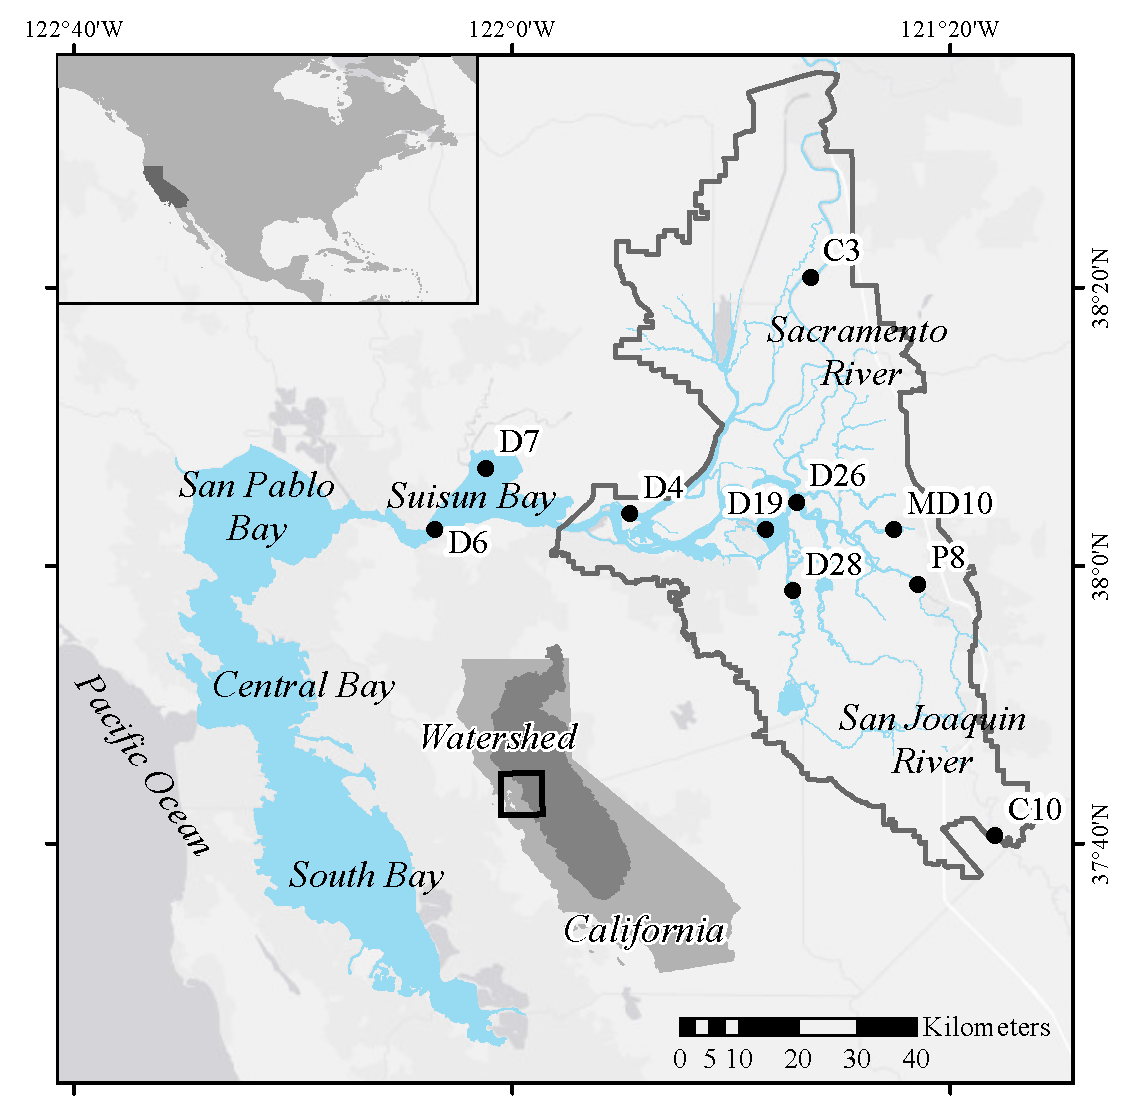
\includegraphics[width=0.8\textwidth,page=1]{figs/delt_map.pdf}
\caption{The \acl{sfe} and Delta region with monitoring stations used for analysis. The Delta drains the combined watersheds of the Sacramento and San Joaquin rivers (inset). All data were obtained from the \acl{iep} website (\url{http://water.ca.gov/bdma/meta/Discrete/data.cfm}, \cite{IEP13}).}
\label{fig:delt_map}   
\end{figure}

\begin{figure}[!ht]

{\centering 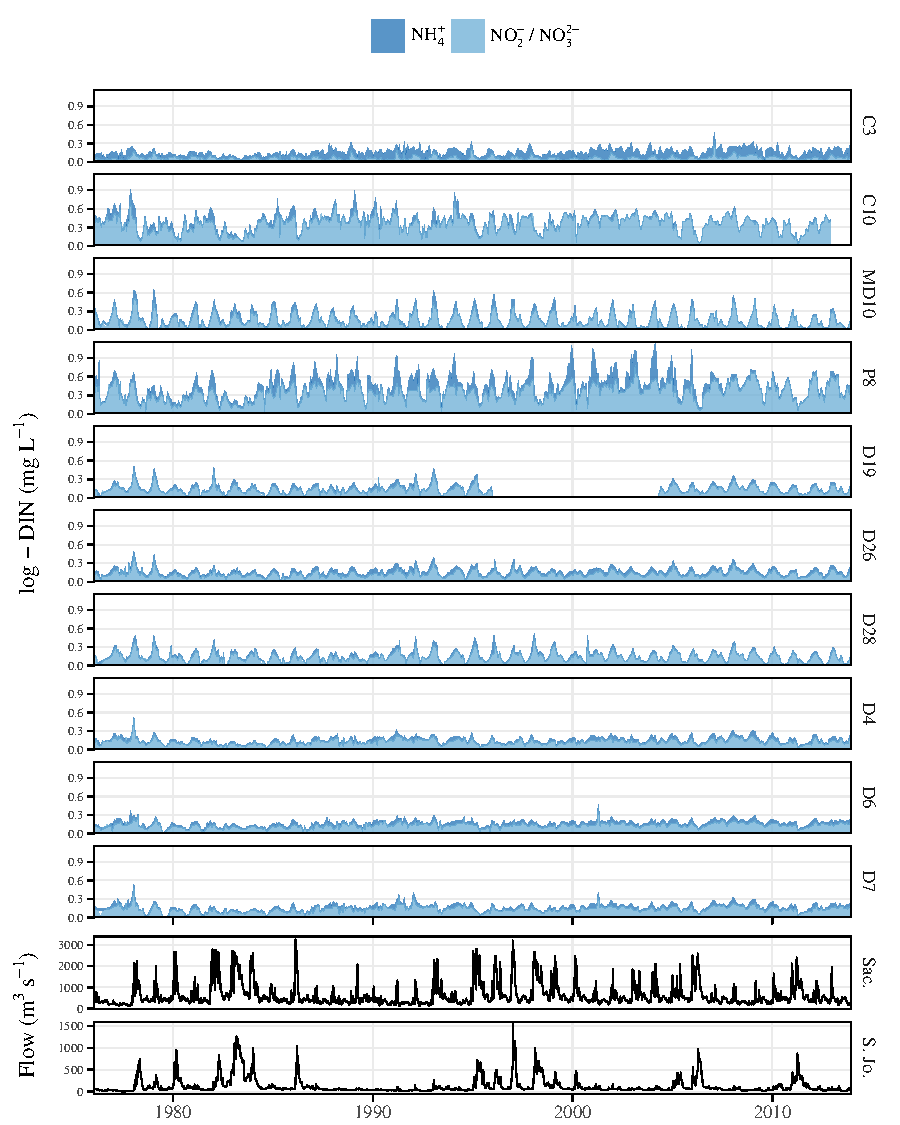
\includegraphics[width=0.9\textwidth]{figs/obsdat-1} 

}

\caption{Observed \ac{din} (NH$_4^{+}$ + NO$_2^{-}$/NO$_3^{2-}$) from ten stations in the upper \ac{sfe} Delta and flow from the Sacramento and San Joaquin rivers.  Data were collected monthly and evaluated with \ac{wrtds} models using daily flow estimates from 1976 to 2013. Note different y-axis scales.  See \cref{fig:delt_map} for station locations.}\label{fig:obsdat}
\end{figure}



\begin{figure}[!ht]

{\centering 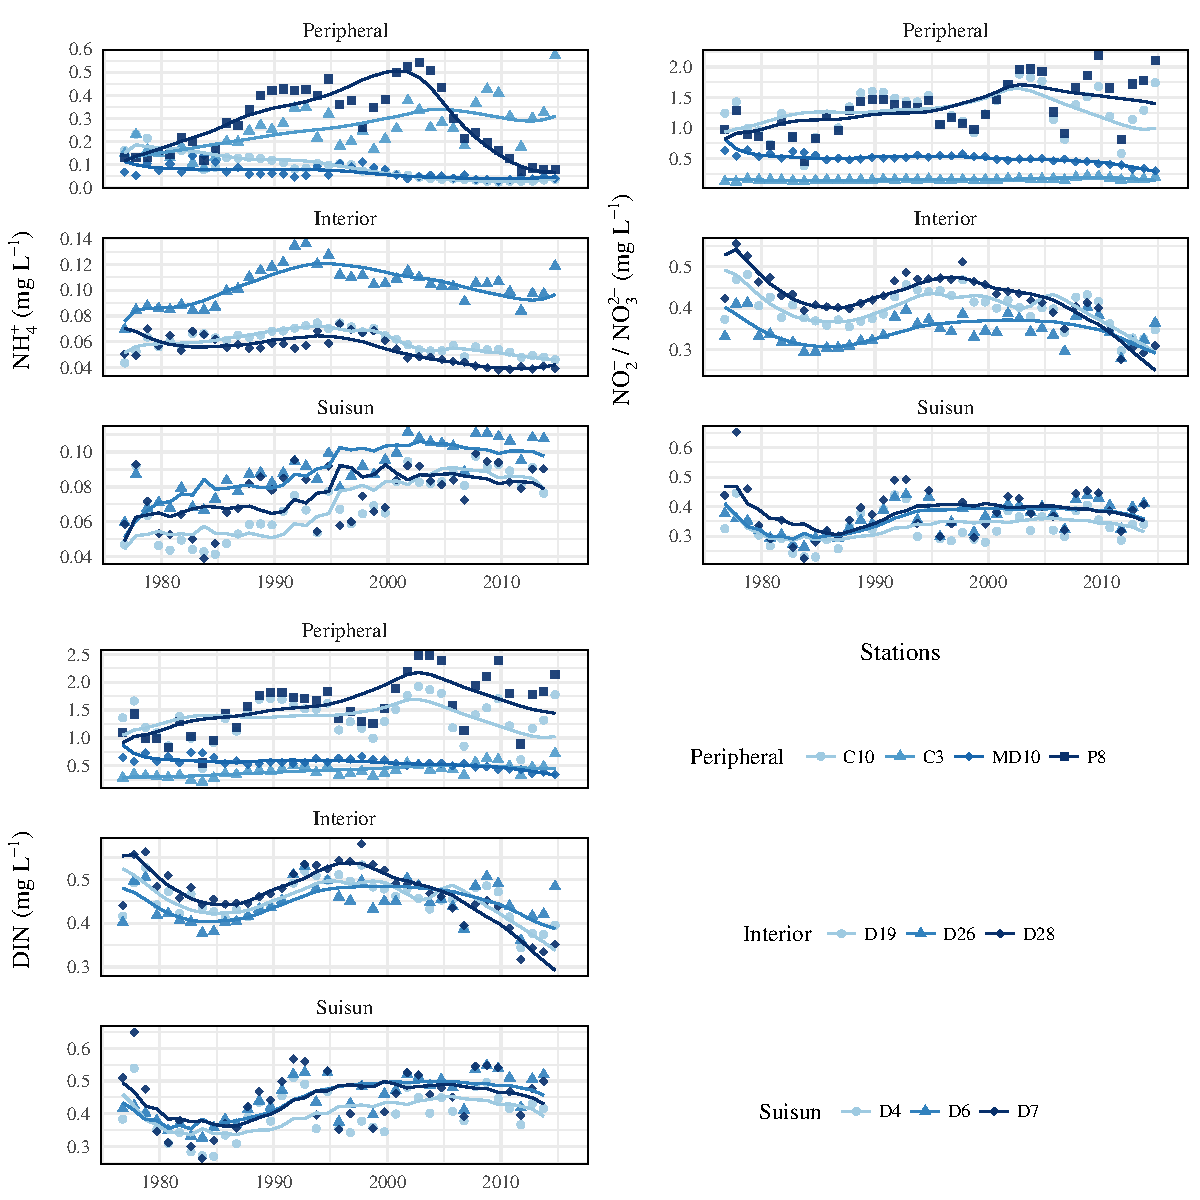
\includegraphics[width=\maxwidth]{figs/prddat-1} 

}

\caption{Model predictions for ten stations grouped by nitrogen analyte and geographic location in the Delta region (locations in \cref{fig:delt_map}).  Results are annually-averaged for each water year from October to September.  Points are model predictions and lines are flow-normalized predictions.}\label{fig:prddat}
\end{figure}





\begin{figure}
\centering
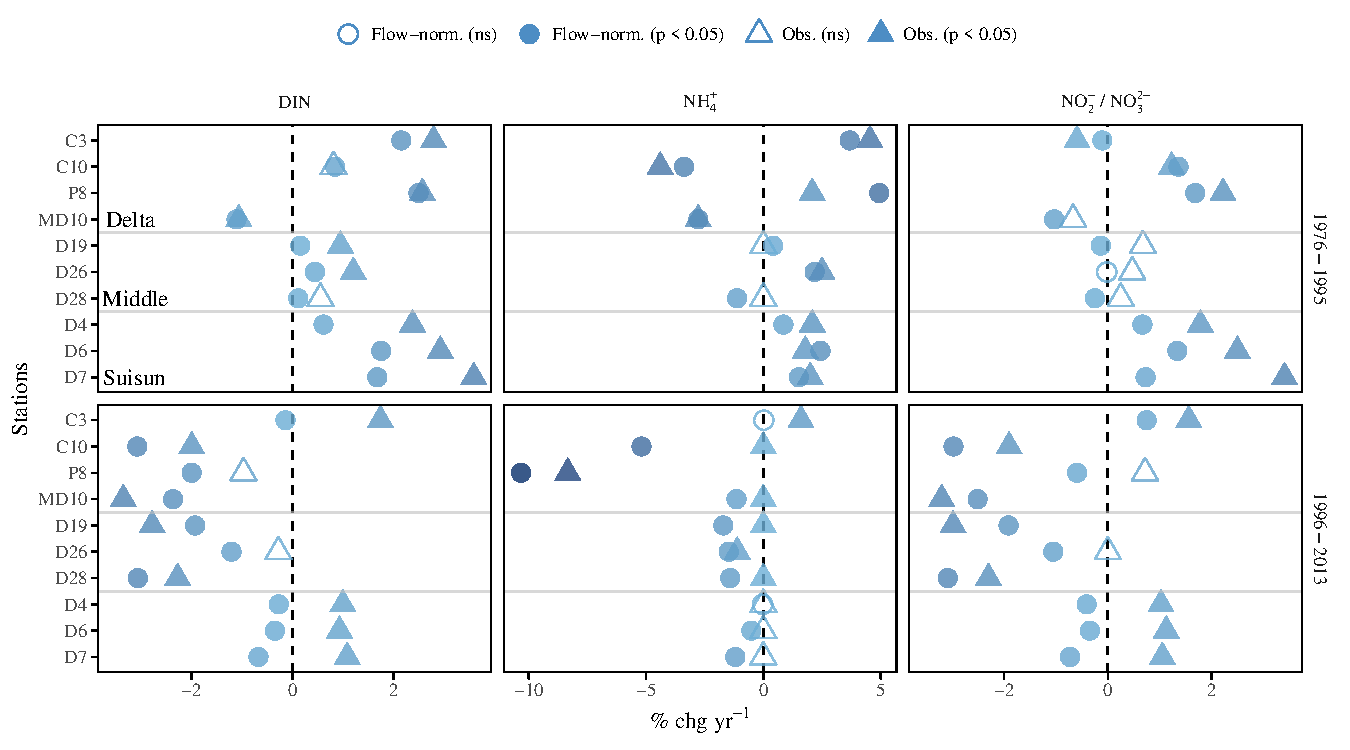
\includegraphics[width=1\textwidth,page=1]{figs/trndcomp1.pdf}
\caption{Results from seasonal Kendall tests on observed data (triangles) and flow-normalized predictions (circles) from \ac{wrtds} for nitrogen analytes. Results are shown as the percent change per year as the estimated Theil-Sen slope divided by the median for a given aggregation period (significance evaluated at $\alpha = 0.05$, based on $\tau$). Trends are shown separately for different annual groupings. See \cref{fig:trndcomp2,fig:trndcomp3} for seasonal groupings.}
\label{fig:trndcomp1}   
\end{figure}

\begin{figure}
\centering
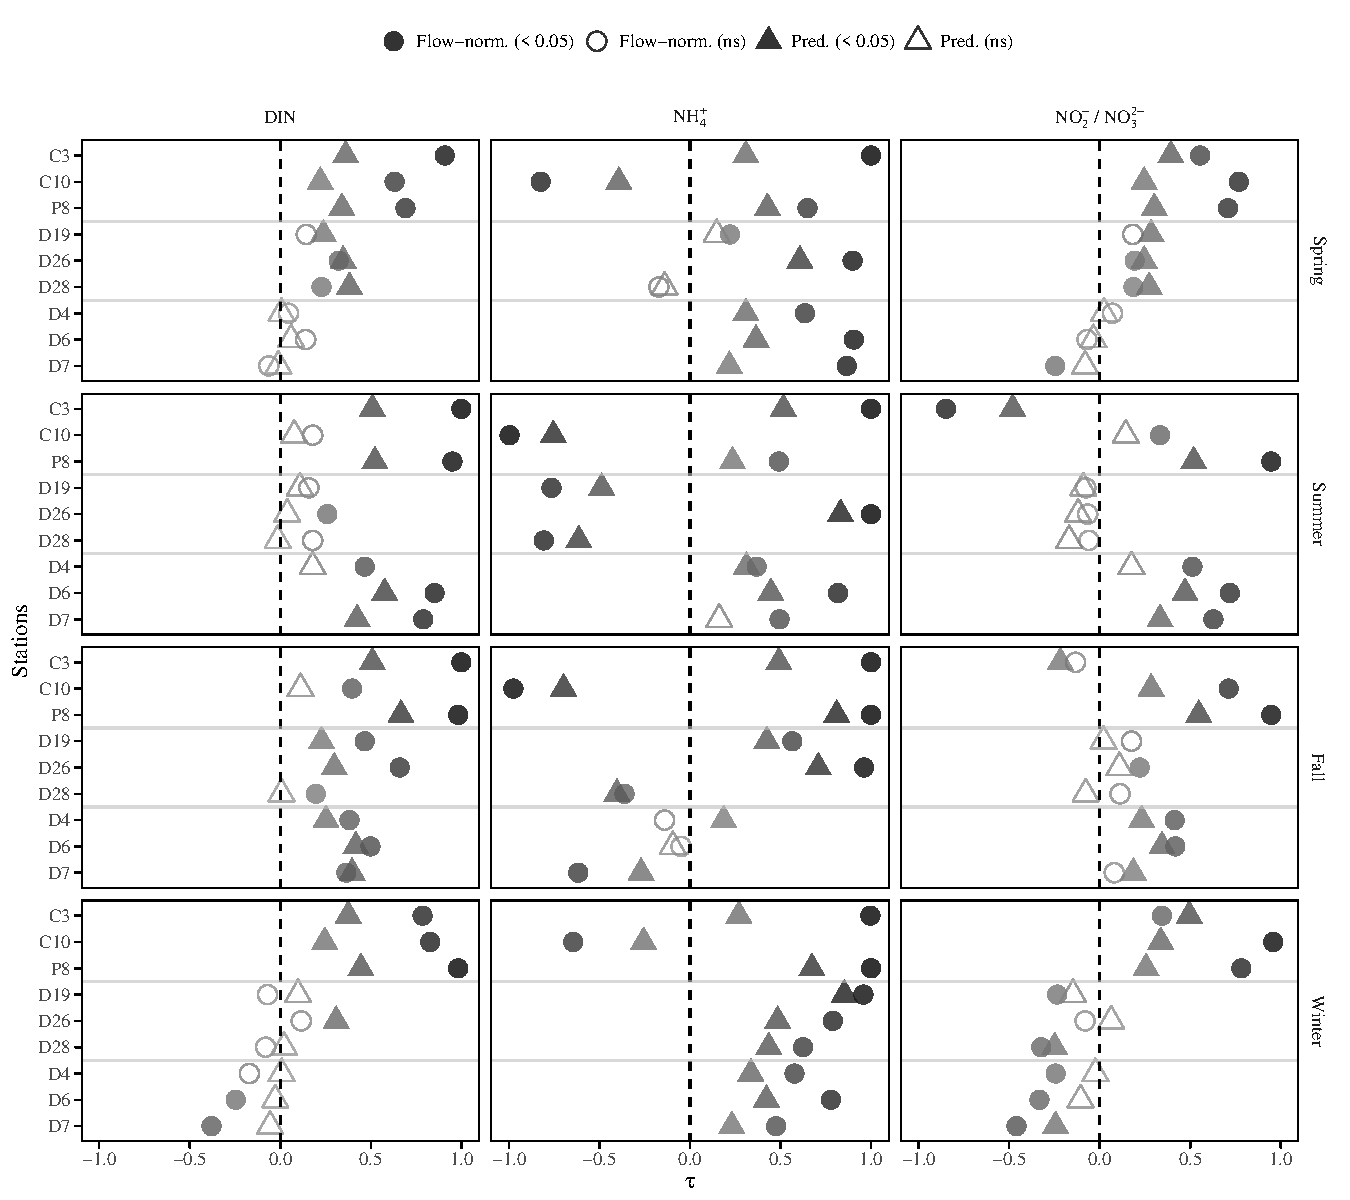
\includegraphics[width=1\textwidth,page=1]{figs/trndcomp2.pdf}
\caption{Results from seasonal Kendall tests on observed data (triangles) and flow-normalized predictions (circles) from \ac{wrtds} for nitrogen analytes. Results are shown as the percent change per year as the estimated Theil-Sen slope divided by the median for a given aggregation period (significance evaluated at $\alpha = 0.05$, based on $\tau$). Trends are shown separately for different seasonal groupings from 1976-1995. Months for each season are Spring: MAM, Summer: JJA, Fall: SON, Winter: DJF. See Figure 3 for annual comparisons.}
\label{fig:trndcomp2}   
\end{figure}

\begin{figure}
\centering
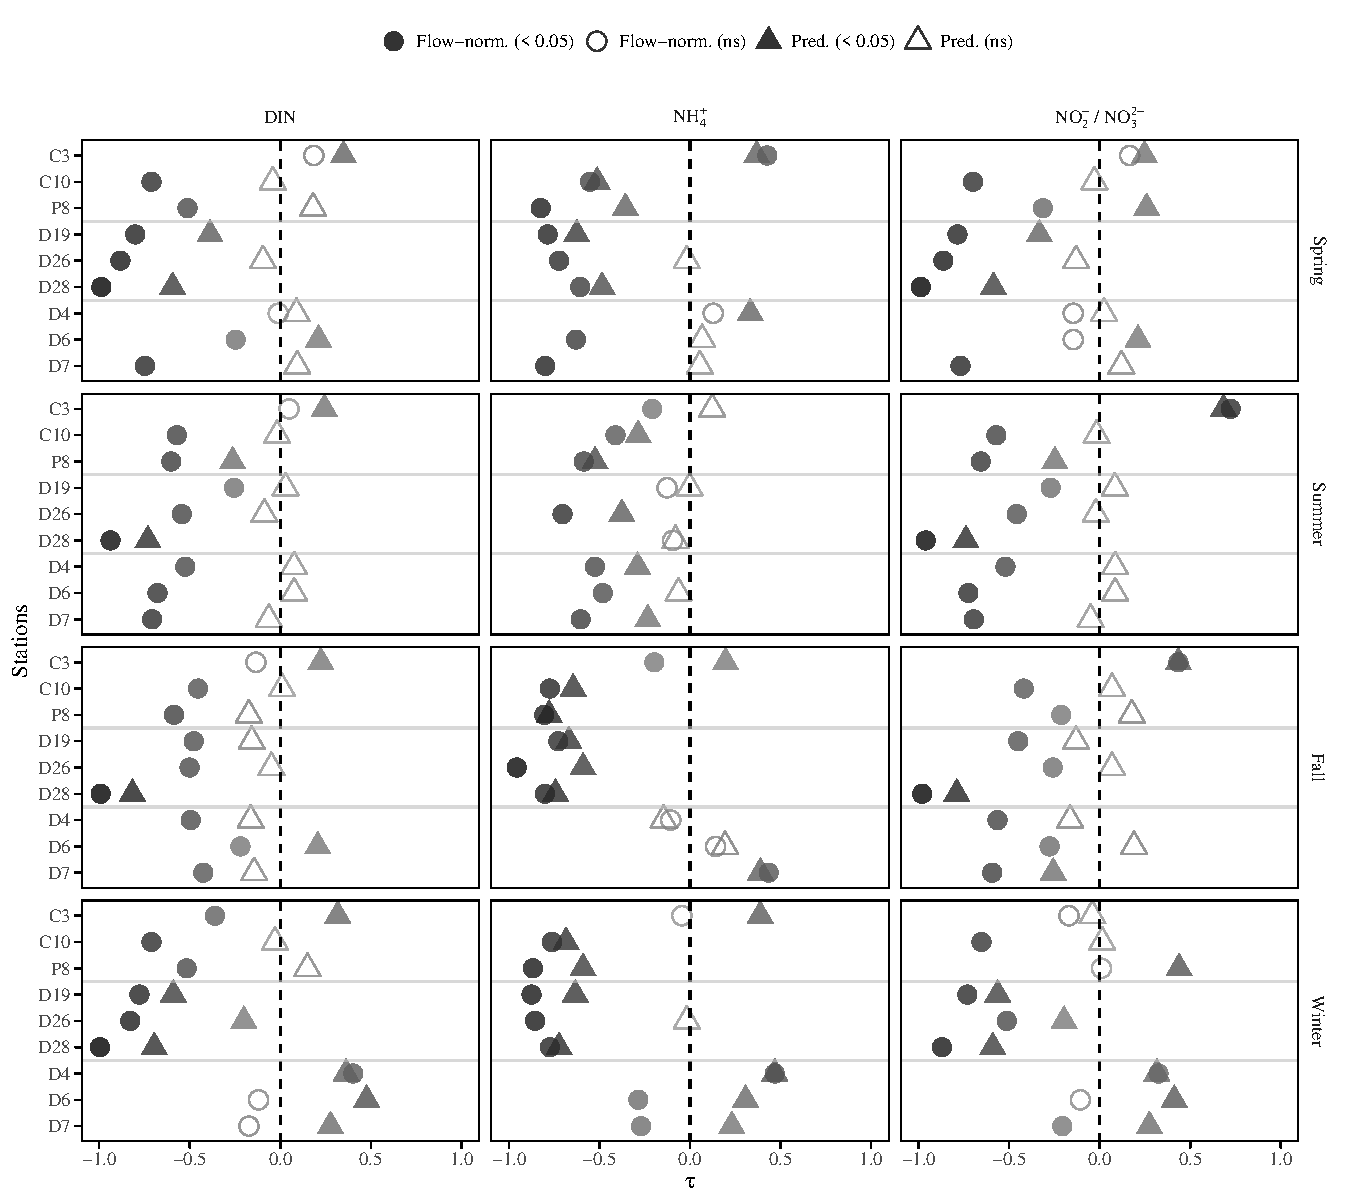
\includegraphics[width=1\textwidth,page=1]{figs/trndcomp3.pdf}
\caption{Results from seasonal Kendall tests on observed data (triangles) and flow-normalized predictions (circles) from \ac{wrtds} for nitrogen analytes. Results are shown as the percent change per year as the estimated Theil-Sen slope divided by the median for a given aggregation period (significance evaluated at $\alpha = 0.05$, based on $\tau$). Trends are shown separately for different seasonal groupings from 1996-2013. Months for each season are Spring: MAM, Summer: JJA, Fall: SON, Winter: DJF. See Figure 3 for annual comparisons.}
\label{fig:trndcomp3}   
\end{figure}

\begin{figure}[!ht]

{\centering 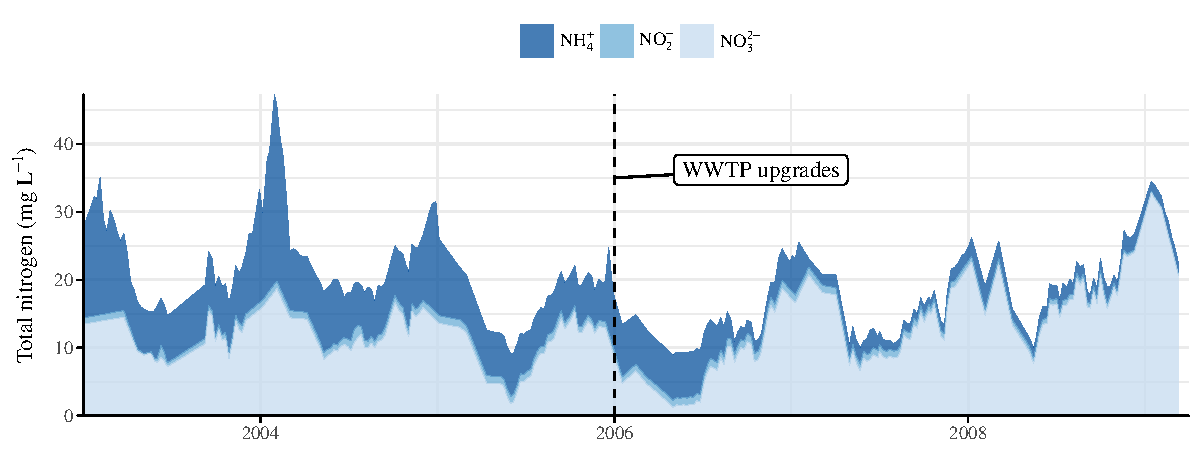
\includegraphics[width=\textwidth]{figs/stock-1} 

}

\caption[Nitrogen concentration measurements (mg L$^{-1}$) from the City of Stockton Wastewater Treatment Plant, San Joaquin County]{Nitrogen concentration measurements (mg L$^{-1}$) from the City of Stockton Wastewater Treatment Plant, San Joaquin County.  Wastewater discharge requirements were implemented in 2006 for nitrification/denitrification and tertiary filtration to convert ammonium to nitrate.}\label{fig:stock}
\end{figure}



\begin{figure}[!ht]

{\centering 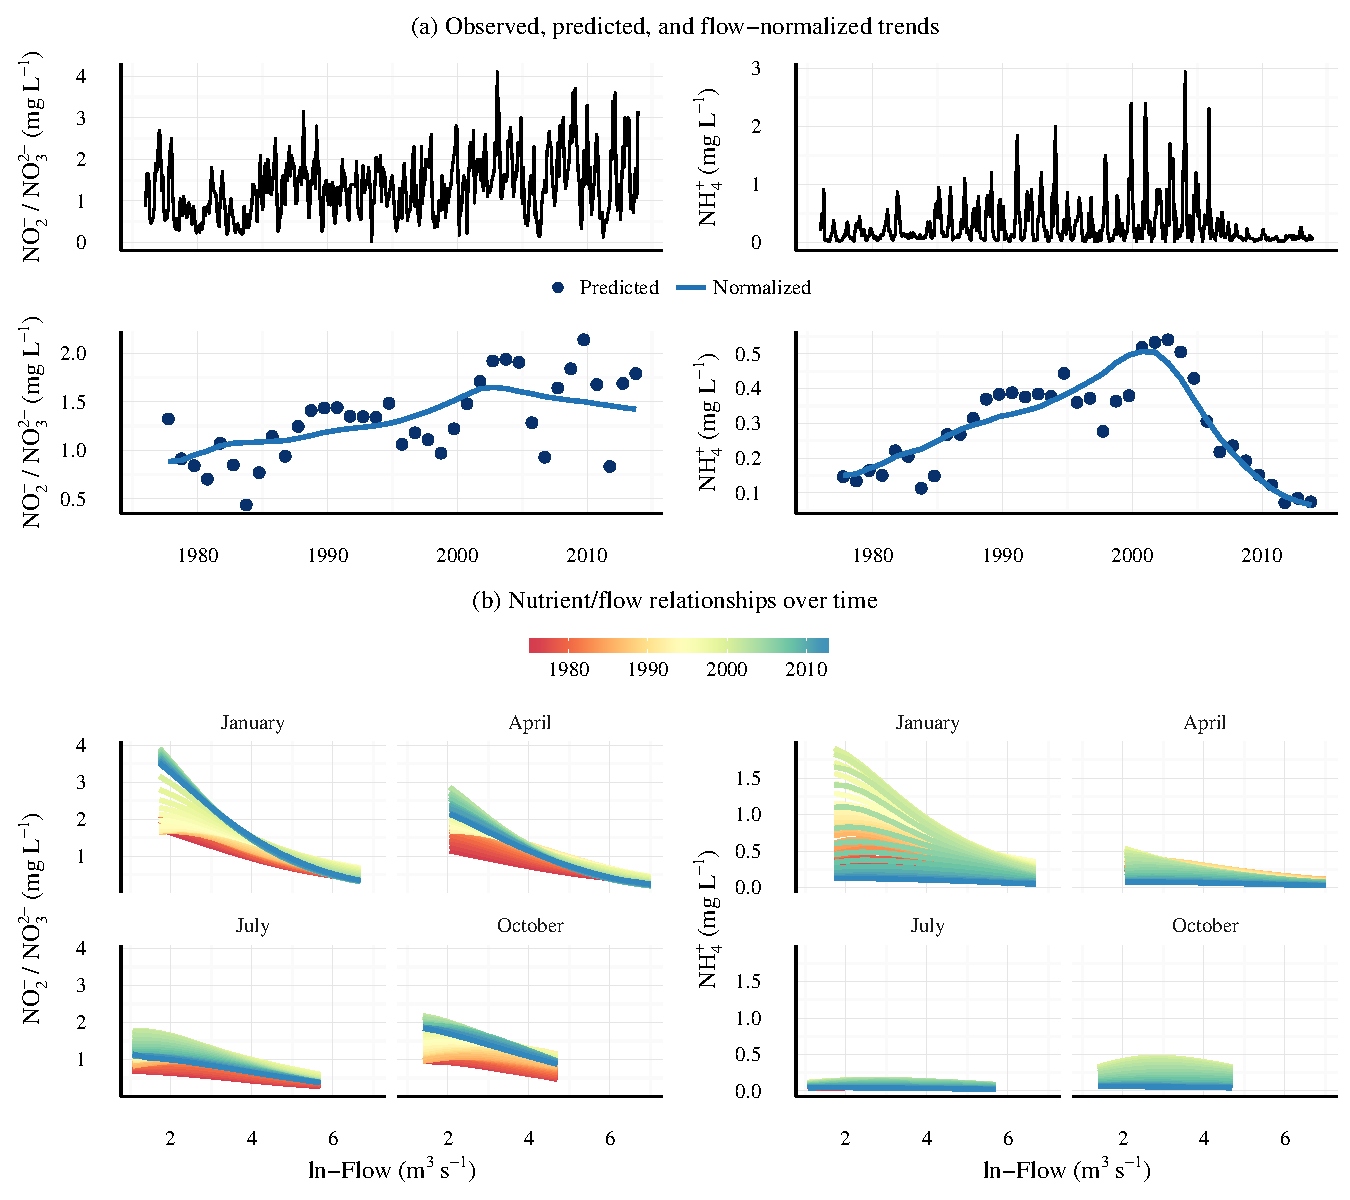
\includegraphics[width=\textwidth]{figs/p8trnds-1} 

}

\caption{Nitrogen trends at P8 as (a, top) observed, (a, bottom) predicted and flow-normalized estimates from \ac{wrtds}, and (b) relationships with flow over time from \ac{wrtds}.  Nitrite/nitrate trends are on the left and ammonium trends are on the right.  Wastewater treatment plant upgrades at the City of Stockton (San Joaquin County) were completed in 2006 (\cref{fig:stock}).}\label{fig:p8trnds}
\end{figure}



\begin{figure}[!ht]

{\centering 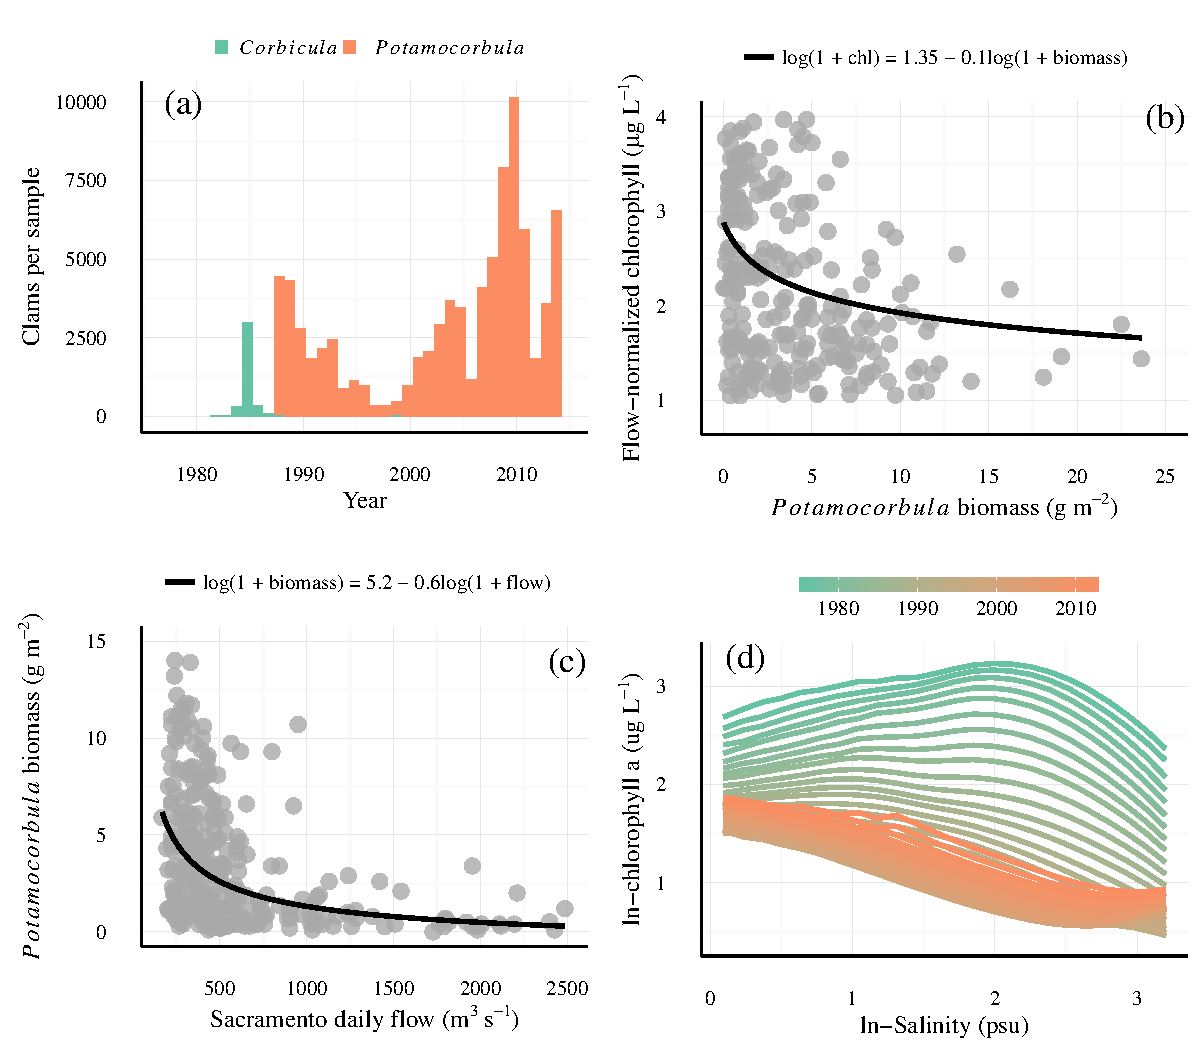
\includegraphics[width=0.9\textwidth]{figs/clmchl-1} 

}

\caption{Trends in clam abundance and \ac{chla} concentration from 1976 to 2013 at station D7 in Suisun Bay.  Invasion by \textit{Potamocorbula amurensis} clams in the late 1980s and reduction of \textit{Corbicula fluminea} was shown by changes in clam density (a, annual means), with biomass linked to salinity (b).  A decrease in \ac{chla} concentration was also observed by changes in annual (c) and seasonal trends (f) based on \ac{wrtds} results.  Reductions in \ac{chla} concentration were coincident with an increase in SiO$_2$ and \ac{din} concentrations (d, e), with the greatest increases in August (g, h). A significant ($p < 0.001$) relationship between clam biomass and \ac{chla} concentration is shown in subfigure (i).  Flow relationships with \ac{chla} concentration shown by \ac{wrtds} have also changed over time (j, observations from June).}\label{fig:clmchl}
\end{figure}



\clearpage
%%%%%%
% tables

% overall trends, years
%latex.default(tab[, -c(1, 2)], file = "", rowlabel = "Analyte/Station",     caption = cap.val, caption.loc = "top", rgroup = vars, n.rgroup = rep(nrow(tab)/3,         3), cgroup = c("Annual"), n.cgroup = c(2), rowname = stats,     label = "tab:trndsann", insert.bottom = foot.val)%
\begin{table}[!tbp]
\caption{Summaries of flow-normalized trends in nitrogen analytes for all stations and annual aggregations\label{tab:trndsann}} 
\begin{center}
\begin{tabular}{lll}
\hline\hline
\multicolumn{1}{l}{\bfseries Analyte/Station}&\multicolumn{2}{c}{\bfseries Annual}\tabularnewline
\cline{2-3}
\multicolumn{1}{l}{}&\multicolumn{1}{c}{1976-1995}&\multicolumn{1}{c}{1996-2013}\tabularnewline
\hline
{\bfseries DIN}&&\tabularnewline
~~C10&1.3 \footnotesize{(\textbf{0.8})*}&1.4 \footnotesize{(-3.1)*}\tabularnewline
~~C3&0.3 \footnotesize{(\textbf{2.2})*}&0.5 \footnotesize{(-0.1)*}\tabularnewline
~~D19&0.4 \footnotesize{(\textbf{0.2})*}&0.4 \footnotesize{(-1.9)*}\tabularnewline
~~D26&0.4 \footnotesize{(\textbf{0.4})*}&0.5 \footnotesize{(-1.2)*}\tabularnewline
~~D28&0.4 \footnotesize{(\textbf{0.1})*}&0.4 \footnotesize{(-3.1)*}\tabularnewline
~~D4&0.3 \footnotesize{(\textbf{0.6})*}&0.4 \footnotesize{(-0.3)*}\tabularnewline
~~D6&0.4 \footnotesize{(\textbf{1.8})*}&0.5 \footnotesize{(-0.3)*}\tabularnewline
~~D7&0.4 \footnotesize{(\textbf{1.7})*}&0.5 \footnotesize{(-0.7)*}\tabularnewline
~~MD10&0.4 \footnotesize{(-1.1)*}&0.3 \footnotesize{(-2.4)*}\tabularnewline
~~P8&1.3 \footnotesize{(\textbf{2.5})*}&1.7 \footnotesize{(-2)*}\tabularnewline
\hline
{\bfseries NH$_{4}^{+}$}&&\tabularnewline
~~C10&0.1 \footnotesize{(-3.4)*}&0 \footnotesize{(-5.2)*}\tabularnewline
~~C3&0.2 \footnotesize{(\textbf{3.7})*}&0.3 \footnotesize{(\textbf{0})}\tabularnewline
~~D19&0 \footnotesize{(\textbf{0.4})*}&0 \footnotesize{(-1.7)*}\tabularnewline
~~D26&0.1 \footnotesize{(\textbf{2.2})*}&0.1 \footnotesize{(-1.5)*}\tabularnewline
~~D28&0 \footnotesize{(-1.1)*}&0 \footnotesize{(-1.4)*}\tabularnewline
~~D4&0 \footnotesize{(\textbf{0.9})*}&0.1 \footnotesize{(\textbf{0})}\tabularnewline
~~D6&0.1 \footnotesize{(\textbf{2.4})*}&0.1 \footnotesize{(-0.5)*}\tabularnewline
~~D7&0.1 \footnotesize{(\textbf{1.5})*}&0.1 \footnotesize{(-1.2)*}\tabularnewline
~~MD10&0.1 \footnotesize{(-2.8)*}&0 \footnotesize{(-1.1)*}\tabularnewline
~~P8&0.2 \footnotesize{(\textbf{4.9})*}&0.1 \footnotesize{(-10.3)*}\tabularnewline
\hline
{\bfseries NO$_{2}^{-}$/NO$_{3}^{2-}$}&&\tabularnewline
~~C10&1.2 \footnotesize{(\textbf{1.4})*}&1.4 \footnotesize{(-3)*}\tabularnewline
~~C3&0.1 \footnotesize{(-0.1)*}&0.2 \footnotesize{(\textbf{0.7})*}\tabularnewline
~~D19&0.4 \footnotesize{(-0.1)*}&0.4 \footnotesize{(-1.9)*}\tabularnewline
~~D26&0.3 \footnotesize{(\textbf{0})}&0.4 \footnotesize{(-1.1)*}\tabularnewline
~~D28&0.4 \footnotesize{(-0.2)*}&0.4 \footnotesize{(-3.1)*}\tabularnewline
~~D4&0.3 \footnotesize{(\textbf{0.7})*}&0.3 \footnotesize{(-0.4)*}\tabularnewline
~~D6&0.3 \footnotesize{(\textbf{1.3})*}&0.4 \footnotesize{(-0.3)*}\tabularnewline
~~D7&0.4 \footnotesize{(\textbf{0.7})*}&0.4 \footnotesize{(-0.7)*}\tabularnewline
~~MD10&0.4 \footnotesize{(-1)*}&0.3 \footnotesize{(-2.5)*}\tabularnewline
~~P8&1.2 \footnotesize{(\textbf{1.7})*}&1.5 \footnotesize{(-0.6)*}\tabularnewline
\hline
\end{tabular}\end{center}
\footnotesize Summaries are  medians (mg L$^{-1}$) and percent change per year in parentheses (increasing in bold). Changes and significance estimates are based on seasonal Kendall tests of flow-normalized results within each time period. *$p<0.05$\end{table}


% overall trends, seasons, first annual periodyears
%latex.default(tab[, -c(1, 2)], file = "", rowlabel = "Analyte/Station",     caption = cap.val, caption.loc = "top", rgroup = vars, n.rgroup = rep(nrow(tab)/3,         3), cgroup = c("Seasonal, 1976-1995"), n.cgroup = c(4),     rowname = stats, label = "tab:trndsbef", insert.bottom = foot.val)%
\begin{table}[!tbp]
\caption{Summaries of flow-normalized trends in nitrogen analytes for all stations and seasonal aggregations from 1976-1995\label{tab:trndsbef}} 
\begin{center}
\begin{tabular}{lllll}
\hline\hline
\multicolumn{1}{l}{\bfseries Analyte/Station}&\multicolumn{4}{c}{\bfseries Seasonal, 1976-1995}\tabularnewline
\cline{2-5}
\multicolumn{1}{l}{}&\multicolumn{1}{c}{Spring}&\multicolumn{1}{c}{Summer}&\multicolumn{1}{c}{Fall}&\multicolumn{1}{c}{Winter}\tabularnewline
\hline
{\bfseries DIN}&&&&\tabularnewline
~~C10&1.2 \footnotesize{(\textbf{1.1})*}&1.2 \footnotesize{(\textbf{0.3})}&1.3 \footnotesize{(\textbf{0.5})*}&1.7 \footnotesize{(\textbf{1.2})*}\tabularnewline
~~C3&0.3 \footnotesize{(\textbf{2.4})*}&0.3 \footnotesize{(\textbf{2.3})*}&0.4 \footnotesize{(\textbf{2.4})*}&0.4 \footnotesize{(\textbf{1.9})*}\tabularnewline
~~D19&0.5 \footnotesize{(\textbf{0.3})}&0.2 \footnotesize{(\textbf{0.4})}&0.3 \footnotesize{(\textbf{0.7})*}&0.7 \footnotesize{(-0.2)}\tabularnewline
~~D26&0.4 \footnotesize{(\textbf{0.7})*}&0.3 \footnotesize{(\textbf{0.4})*}&0.4 \footnotesize{(\textbf{1})*}&0.6 \footnotesize{(\textbf{0.3})}\tabularnewline
~~D28&0.5 \footnotesize{(\textbf{0.8})*}&0.2 \footnotesize{(\textbf{0.3})}&0.3 \footnotesize{(\textbf{0.5})*}&0.8 \footnotesize{(-0.3)}\tabularnewline
~~D4&0.4 \footnotesize{(\textbf{0.2})}&0.3 \footnotesize{(\textbf{1.4})*}&0.3 \footnotesize{(\textbf{1.1})*}&0.5 \footnotesize{(-0.5)}\tabularnewline
~~D6&0.4 \footnotesize{(\textbf{0.4})}&0.3 \footnotesize{(\textbf{4.6})*}&0.4 \footnotesize{(\textbf{1.4})*}&0.5 \footnotesize{(-0.7)*}\tabularnewline
~~D7&0.4 \footnotesize{(-0.2)}&0.3 \footnotesize{(\textbf{4.2})*}&0.4 \footnotesize{(\textbf{1.5})*}&0.6 \footnotesize{(-2.4)*}\tabularnewline
~~MD10&0.6 \footnotesize{(-0.3)}&0.2 \footnotesize{(-3.6)*}&0.3 \footnotesize{(\textbf{0.8})*}&1.3 \footnotesize{(-0.3)*}\tabularnewline
~~P8&1.3 \footnotesize{(\textbf{2.4})*}&0.9 \footnotesize{(\textbf{2.4})*}&1.3 \footnotesize{(\textbf{3.1})*}&1.9 \footnotesize{(\textbf{2.1})*}\tabularnewline
\hline
{\bfseries NH$_{4}^{+}$}&&&&\tabularnewline
~~C10&0.1 \footnotesize{(-2.3)*}&0 \footnotesize{(-6.8)*}&0.1 \footnotesize{(-7.1)*}&0.3 \footnotesize{(-1.5)*}\tabularnewline
~~C3&0.2 \footnotesize{(\textbf{3.9})*}&0.2 \footnotesize{(\textbf{4})*}&0.3 \footnotesize{(\textbf{3.8})*}&0.2 \footnotesize{(\textbf{2.9})*}\tabularnewline
~~D19&0.1 \footnotesize{(\textbf{0.4})*}&0 \footnotesize{(-1.7)*}&0 \footnotesize{(\textbf{1.2})*}&0.1 \footnotesize{(\textbf{2.5})*}\tabularnewline
~~D26&0.1 \footnotesize{(\textbf{1.4})*}&0.1 \footnotesize{(\textbf{2.5})*}&0.1 \footnotesize{(\textbf{3.1})*}&0.1 \footnotesize{(\textbf{2.3})*}\tabularnewline
~~D28&0.1 \footnotesize{(-0.5)}&0 \footnotesize{(-3.7)*}&0 \footnotesize{(-1.6)*}&0.1 \footnotesize{(\textbf{1.7})*}\tabularnewline
~~D4&0.1 \footnotesize{(\textbf{1.7})*}&0 \footnotesize{(\textbf{1})*}&0 \footnotesize{(-0.7)}&0.1 \footnotesize{(\textbf{2})*}\tabularnewline
~~D6&0.1 \footnotesize{(\textbf{2.9})*}&0.1 \footnotesize{(\textbf{2.8})*}&0.1 \footnotesize{(-0.1)}&0.1 \footnotesize{(\textbf{2.1})*}\tabularnewline
~~D7&0.1 \footnotesize{(\textbf{3.3})*}&0 \footnotesize{(\textbf{2})*}&0.1 \footnotesize{(-2.8)*}&0.1 \footnotesize{(\textbf{1.7})*}\tabularnewline
~~MD10&0.1 \footnotesize{(-1.8)*}&0 \footnotesize{(-6.5)*}&0 \footnotesize{(-3.3)*}&0.2 \footnotesize{(\textbf{0.4})}\tabularnewline
~~P8&0.2 \footnotesize{(\textbf{3.9})*}&0.1 \footnotesize{(\textbf{1.8})*}&0.2 \footnotesize{(\textbf{7})*}&0.6 \footnotesize{(\textbf{7})*}\tabularnewline
\hline
{\bfseries NO$_{2}^{-}$/NO$_{3}^{2-}$}&&&&\tabularnewline
~~C10&1.1 \footnotesize{(\textbf{1.5})*}&1.2 \footnotesize{(\textbf{0.6})*}&1.2 \footnotesize{(\textbf{1.3})*}&1.5 \footnotesize{(\textbf{1.8})*}\tabularnewline
~~C3&0.2 \footnotesize{(\textbf{0.7})*}&0.1 \footnotesize{(-1)*}&0.1 \footnotesize{(-0.3)}&0.2 \footnotesize{(\textbf{1})*}\tabularnewline
~~D19&0.4 \footnotesize{(\textbf{0.4})}&0.2 \footnotesize{(-0.3)}&0.3 \footnotesize{(\textbf{0.3})}&0.6 \footnotesize{(-0.9)*}\tabularnewline
~~D26&0.4 \footnotesize{(\textbf{0.6})*}&0.2 \footnotesize{(-0.1)}&0.3 \footnotesize{(\textbf{0.3})*}&0.5 \footnotesize{(-0.3)}\tabularnewline
~~D28&0.5 \footnotesize{(\textbf{0.7})*}&0.2 \footnotesize{(-0.1)}&0.3 \footnotesize{(\textbf{0.2})}&0.7 \footnotesize{(-1)*}\tabularnewline
~~D4&0.3 \footnotesize{(\textbf{0.1})}&0.3 \footnotesize{(\textbf{1.4})*}&0.3 \footnotesize{(\textbf{1.1})*}&0.4 \footnotesize{(-0.8)*}\tabularnewline
~~D6&0.4 \footnotesize{(-0.2)}&0.3 \footnotesize{(\textbf{4.1})*}&0.3 \footnotesize{(\textbf{1.4})*}&0.4 \footnotesize{(-1)*}\tabularnewline
~~D7&0.4 \footnotesize{(-1)*}&0.3 \footnotesize{(\textbf{3.4})*}&0.4 \footnotesize{(\textbf{0.4})}&0.4 \footnotesize{(-3.6)*}\tabularnewline
~~MD10&0.5 \footnotesize{(-0.2)}&0.2 \footnotesize{(-3.6)*}&0.2 \footnotesize{(\textbf{1.5})*}&1.2 \footnotesize{(-0.5)*}\tabularnewline
~~P8&1.2 \footnotesize{(\textbf{2})*}&0.9 \footnotesize{(\textbf{2.3})*}&1.1 \footnotesize{(\textbf{2})*}&1.4 \footnotesize{(\textbf{1})*}\tabularnewline
\hline
\end{tabular}\end{center}
\footnotesize Summaries are  medians (mg L$^{-1}$) and percent change per year in parentheses (increasing in bold). Changes and significance estimates are based on seasonal Kendall tests of flow-normalized results within each time period. Months for each season are Spring: MAM, Summer: JJA, Fall: SON, Winter: DJF. *$p<0.05$\end{table}


% overall trends, seasons, first annual periodyears
%latex.default(tab[, -c(1, 2)], file = "", rowlabel = "Analyte/Station",     caption = cap.val, caption.loc = "top", rgroup = vars, n.rgroup = rep(nrow(tab)/3,         3), cgroup = c("Seasonal, 1996-2013"), n.cgroup = c(4),     rowname = stats, label = "tab:trndsaft", insert.bottom = foot.val)%
\begin{table}[!tbp]
\caption{Summaries of flow-normalized trends in nitrogen analytes for all stations and seasonal aggregations from 1996-2013\label{tab:trndsaft}} 
\begin{center}
\begin{tabular}{lllll}
\hline\hline
\multicolumn{1}{l}{\bfseries Analyte/Station}&\multicolumn{4}{c}{\bfseries Seasonal, 1996-2013}\tabularnewline
\cline{2-5}
\multicolumn{1}{l}{}&\multicolumn{1}{c}{Spring}&\multicolumn{1}{c}{Summer}&\multicolumn{1}{c}{Fall}&\multicolumn{1}{c}{Winter}\tabularnewline
\hline
{\bfseries DIN}&&&&\tabularnewline
~~C10&1.1 \footnotesize{(-4.1)*}&1.3 \footnotesize{(-3.1)*}&1.6 \footnotesize{(-2)*}&1.7 \footnotesize{(-3.4)*}\tabularnewline
~~C3&0.5 \footnotesize{(\textbf{0.5})}&0.4 \footnotesize{(\textbf{0.1})}&0.6 \footnotesize{(-0.2)}&0.5 \footnotesize{(-0.6)*}\tabularnewline
~~D19&0.5 \footnotesize{(-2.8)*}&0.2 \footnotesize{(-1)*}&0.3 \footnotesize{(-1.6)*}&0.7 \footnotesize{(-2.3)*}\tabularnewline
~~D26&0.5 \footnotesize{(-1.9)*}&0.3 \footnotesize{(-1.7)*}&0.4 \footnotesize{(-1)*}&0.6 \footnotesize{(-0.8)*}\tabularnewline
~~D28&0.5 \footnotesize{(-3)*}&0.2 \footnotesize{(-4.9)*}&0.2 \footnotesize{(-4.9)*}&0.7 \footnotesize{(-2.1)*}\tabularnewline
~~D4&0.4 \footnotesize{(\textbf{0})}&0.4 \footnotesize{(-1)*}&0.4 \footnotesize{(-0.9)*}&0.5 \footnotesize{(\textbf{0.6})*}\tabularnewline
~~D6&0.5 \footnotesize{(-0.2)*}&0.5 \footnotesize{(-1)*}&0.5 \footnotesize{(-0.3)*}&0.5 \footnotesize{(-0.1)}\tabularnewline
~~D7&0.5 \footnotesize{(-0.8)*}&0.4 \footnotesize{(-1.3)*}&0.4 \footnotesize{(-0.4)*}&0.6 \footnotesize{(-0.2)}\tabularnewline
~~MD10&0.4 \footnotesize{(-2.3)*}&0.2 \footnotesize{(-3.7)*}&0.2 \footnotesize{(-4.4)*}&1 \footnotesize{(-1.8)*}\tabularnewline
~~P8&1.5 \footnotesize{(-1.9)*}&1.2 \footnotesize{(-3.5)*}&1.8 \footnotesize{(-2.4)*}&2.7 \footnotesize{(-2.2)*}\tabularnewline
\hline
{\bfseries NH$_{4}^{+}$}&&&&\tabularnewline
~~C10&0 \footnotesize{(-4.2)*}&0 \footnotesize{(-6.1)*}&0 \footnotesize{(-8.5)*}&0.1 \footnotesize{(-7.3)*}\tabularnewline
~~C3&0.3 \footnotesize{(\textbf{1})*}&0.3 \footnotesize{(-0.8)*}&0.4 \footnotesize{(-0.5)*}&0.2 \footnotesize{(-0.1)}\tabularnewline
~~D19&0 \footnotesize{(-1.9)*}&0 \footnotesize{(-0.4)}&0 \footnotesize{(-2.2)*}&0.1 \footnotesize{(-1.8)*}\tabularnewline
~~D26&0.1 \footnotesize{(-1.2)*}&0.1 \footnotesize{(-1.3)*}&0.1 \footnotesize{(-1.9)*}&0.1 \footnotesize{(-1.4)*}\tabularnewline
~~D28&0 \footnotesize{(-1.7)*}&0 \footnotesize{(-0.2)}&0 \footnotesize{(-2.4)*}&0.1 \footnotesize{(-3.1)*}\tabularnewline
~~D4&0.1 \footnotesize{(\textbf{0.3})}&0 \footnotesize{(-1.3)*}&0.1 \footnotesize{(-0.3)}&0.1 \footnotesize{(\textbf{1})*}\tabularnewline
~~D6&0.1 \footnotesize{(-0.7)*}&0.1 \footnotesize{(-1)*}&0.1 \footnotesize{(\textbf{0.3})}&0.1 \footnotesize{(-0.3)*}\tabularnewline
~~D7&0.1 \footnotesize{(-2.2)*}&0 \footnotesize{(-2.1)*}&0.1 \footnotesize{(\textbf{1.3})*}&0.1 \footnotesize{(-0.4)*}\tabularnewline
~~MD10&0 \footnotesize{(-1.4)*}&0 \footnotesize{(-0.1)}&0 \footnotesize{(-0.8)*}&0.1 \footnotesize{(-4.3)*}\tabularnewline
~~P8&0.2 \footnotesize{(-8.7)*}&0.1 \footnotesize{(-6.3)*}&0.2 \footnotesize{(-10.4)*}&0.5 \footnotesize{(-13.1)*}\tabularnewline
\hline
{\bfseries NO$_{2}^{-}$/NO$_{3}^{2-}$}&&&&\tabularnewline
~~C10&1.1 \footnotesize{(-4.2)*}&1.2 \footnotesize{(-3.2)*}&1.6 \footnotesize{(-1.9)*}&1.6 \footnotesize{(-3.3)*}\tabularnewline
~~C3&0.2 \footnotesize{(\textbf{0.4})}&0.1 \footnotesize{(\textbf{3.1})*}&0.2 \footnotesize{(\textbf{1.7})*}&0.2 \footnotesize{(-0.4)}\tabularnewline
~~D19&0.4 \footnotesize{(-2.9)*}&0.2 \footnotesize{(-1)*}&0.3 \footnotesize{(-1.5)*}&0.6 \footnotesize{(-2.2)*}\tabularnewline
~~D26&0.4 \footnotesize{(-1.9)*}&0.2 \footnotesize{(-1.6)*}&0.3 \footnotesize{(-0.6)*}&0.5 \footnotesize{(-0.6)*}\tabularnewline
~~D28&0.5 \footnotesize{(-3)*}&0.2 \footnotesize{(-5.4)*}&0.2 \footnotesize{(-5.2)*}&0.7 \footnotesize{(-1.7)*}\tabularnewline
~~D4&0.3 \footnotesize{(-0.1)}&0.3 \footnotesize{(-1)*}&0.3 \footnotesize{(-1)*}&0.4 \footnotesize{(\textbf{0.4})*}\tabularnewline
~~D6&0.4 \footnotesize{(-0.1)}&0.4 \footnotesize{(-1)*}&0.4 \footnotesize{(-0.4)*}&0.4 \footnotesize{(-0.1)}\tabularnewline
~~D7&0.4 \footnotesize{(-0.6)*}&0.4 \footnotesize{(-1.2)*}&0.4 \footnotesize{(-0.8)*}&0.4 \footnotesize{(-0.3)*}\tabularnewline
~~MD10&0.4 \footnotesize{(-2.6)*}&0.1 \footnotesize{(-4.5)*}&0.2 \footnotesize{(-5.4)*}&1 \footnotesize{(-1.4)*}\tabularnewline
~~P8&1.3 \footnotesize{(-1.1)*}&1.1 \footnotesize{(-3.1)*}&1.6 \footnotesize{(-0.3)*}&2.2 \footnotesize{(\textbf{0})}\tabularnewline
\hline
\end{tabular}\end{center}
\footnotesize Summaries are  medians (mg L$^{-1}$) and percent change per year in parentheses (increasing in bold). Changes and significance estimates are based on seasonal Kendall tests of flow-normalized results within each time period. Months for each season are Spring: MAM, Summer: JJA, Fall: SON, Winter: DJF. *$p<0.05$\end{table}


% trends in no23, nh at p8
%latex.default(totab, file = "", rowlabel = "Period", caption = cap.val,     caption.loc = "top", rgroup = segs, n.rgroup = c(2, rep(4,         2)), cgroup = vars, n.cgroup = c(2, 2), rowname = cats,     label = "tab:p8chg", insert.bottom = foot.val)%
\begin{table}[!tbp]
\caption{Summaries of flow-normalized trends in nitrite/nitrate and ammonium (mg L$^{-1}$) concentrations before and after \ac{wwtp} upgrades upstream of station P8\label{tab:p8chg}} 
\begin{center}
\begin{tabular}{lllcll}
\hline\hline
\multicolumn{1}{l}{\bfseries Period}&\multicolumn{2}{c}{\bfseries NO$_{2}^{-}$/NO$_{3}^{2-}$}&\multicolumn{1}{c}{\bfseries }&\multicolumn{2}{c}{\bfseries NH$_{4}^{+}$}\tabularnewline
\cline{2-3} \cline{5-6}
\multicolumn{1}{l}{}&\multicolumn{1}{c}{Median}&\multicolumn{1}{c}{\% change}&\multicolumn{1}{c}{}&\multicolumn{1}{c}{Median}&\multicolumn{1}{c}{\% change}\tabularnewline
\hline
{\bfseries Annual}&&&&&\tabularnewline
~~1976-2006&1.3&\textbf{2}*&&0.2&\textbf{2.8}*\tabularnewline
~~2007-2013&1.4&-1.9*&&0.1&-16.6*\tabularnewline
\hline
{\bfseries Seasonal, pre}&&&&&\tabularnewline
~~Spring&1.2&\textbf{1.6}*&&0.2&\textbf{1.4}*\tabularnewline
~~Summer&1&\textbf{2.4}*&&0.1&\textbf{3.3}*\tabularnewline
~~Fall&1.3&\textbf{2.2}*&&0.2&\textbf{4.9}*\tabularnewline
~~Winter&1.5&\textbf{2.1}*&&0.7&\textbf{4.8}*\tabularnewline
\hline
{\bfseries Seasonal, post}&&&&&\tabularnewline
~~Spring&1.3&-1.6*&&0.1&-16.2*\tabularnewline
~~Summer&0.9&-4.3*&&0.1&-15.7*\tabularnewline
~~Fall&1.5&-1.7*&&0.1&-19.3*\tabularnewline
~~Winter&2.2&-0.8*&&0.2&-26.7*\tabularnewline
\hline
\end{tabular}\end{center}
\footnotesize Upgrades were completed in 2006 at the City of Stockton \ac{wwtp} (San Joaquin County, \cref{fig:stock}). Summaries are  medians and percent change per year in parentheses (increasing in bold).  Changes and significance estimates are based on seasonal Kendall tests of flow-normalized results within each time period. Increasing values are in bold-italics. Months for each season are Spring: MAM, Summer: JJA, Fall: SON, Winter: DJF. *$p<0.05$\end{table}


\clearpage

\end{document}
